\documentclass[12pt]{article}
\usepackage{pifont}
\usepackage{a4wide}
\usepackage[utf8x]{inputenc}
\usepackage{amsmath}
\usepackage{amsfonts}
\usepackage{mathrsfs}
%\usepackage{natbib}
\usepackage{graphicx} % figuras
%\usepackage[export]{adjustbox} % loads also graphicx
\usepackage{float}
\usepackage[font=footnotesize]{caption}
\usepackage{wrapfig}
\usepackage{authblk}
\usepackage{subfigure}

\usepackage{amssymb}
\usepackage{latexsym}
\usepackage[sort&compress]{natbib}



\topmargin=-2pt
\title{On POD-based Deflation Vectors for DPCG applied to porous media problems.}

\author[1]{G. B. Diaz Cortes}  
\author[1]{C. Vuik} 
\author[2]{J. D. Jansen} 
\affil[1]{Department of Applied Mathematics, TU Delft}
\affil[2]{Department of Geoscience \& Engineering, TU Delft}
\renewcommand\Authands{ and }
%\date{April 2017}


\begin{document}
% \thispagestyle{empty}
% \noindent
% \begin{center}
% {\Large \sc DELFT UNIVERSITY OF TECHNOLOGY}
% \\
% \vspace{3cm}
% {\large \sc REPORT 17-01}\\[4ex]
% {\large \sc On POD-based Deflation Vectors for DPCG applied to porous media problems.}\\[4ex]
% {\large \sc G. B. Diaz Cortes, C. Vuik, J. D. Jansen}\\
% \vfill
% {\tt ISSN 1389-6520}\\[2ex]
% {\tt Reports of the Delft Institute of Applied Mathematics}\\[2ex]
% {\tt Delft 2017}
% \end{center}
% \pagebreak
% \thispagestyle{empty}
% \vspace*{\fill}
% \noindent
% \hspace*{-0,3cm}Copyright~~~\Pisymbol{psy}{227}~~~2017 by Delft Institute of Applied Mathematics, Delft, \mbox{The Netherlands.}
% \\[2ex]
% No part of the Journal may be reproduced, stored in a retrieval system, or
% transmitted, in any form or by any means, electronic, mechanical, photocopying,
% recording, or otherwise, without the prior written permission from Delft Institute of
% Applied Mathematics, Delft University of Technology, The
% Netherlands. 
% % newpage, title etc.
% \setcounter{page}{1}
\newpage
\maketitle
\begin{abstract}
      Simulation of two-phase flow trough highly heterogeneous porous media results in large systems of linear equations for the pressure equation, when using e.g., sequential procedures.
      During simulation, the most time consuming part is the solution of the resulting linear system. In this work, solution of the elliptic pressure equation is studied with preconditioning and deflation techniques based on information obtained from the system.\\
      For good performance of deflation techniques, it is necessary to find good deflation vectors. If a good selection of these vectors is made, only a a small increase in the required computing time per iteration and an important decrease in the number of iterations is achieved.  \\
     In this work, we propose the capture of a series of snapshots, solutions of the system, and the use of them as deflation vectors. These snapshots are used directly as deflation vectors and to construct a POD basis. A POD-reduced basis is also proposed as deflation vectors. We investigate convergence and the properties of the resulting methods. 
     We perform a series of numerical experiments with diverse conditions.  
 We consider compressible two-phase flow in a layered model with variations in the permeability layers up to $10^{3}$ and the SPE 10 benchmark model with a contrast in permeability coefficients of $10^{7}$. We study 2D and 3D reservoirs, taking into account gravity terms for the 3D case. We consider immiscible fluids with and without capillary pressure. We studied water flooding, with injection through the boundaries and through wells.
 %For most of the problems solved with deflation, the number of iterations is reduced up to $\sim 80\%$ when compared with the only-preconditioned solver.\\
\end{abstract}
\newpage
\section{Introduction}
 \subsection{Two phase flow through porous media}\label{fpm}
When simulating two phase flow through a porous medium, these two phases can be considered as separated, i.e., they are immiscible and there is no mass transfer between them. 
The contact area between the phases is known as the interface.\\ 
When modeling two phases, we 
usually consider one of the fluids as the wetting phase ($w$), which is more attracted to the mineral particles than the other phase.
The other phase is considered as non-wetting phase ($n$). In the case of a water-oil system, water is considered
the wetting phase. \\
% For a reservoir, the density of each phase varies, the gas is less dense than the oil and water. 
% Therefore, the gas is found on top of the reservoir. For the oil-water system, water's density is larger 
% than oil's, then water is found on the bottom of the reservoir.\\
The saturation of a phase $(S_{\alpha}),$ is the fraction of void space filled with that phase in the 
medium, where a zero saturation indicates that the phase is not present.
If there are two phases present in the porous medium, these fluids fill completely the empty space, which is
expressed by the following relation,
\begin{equation}\label{eq:satrel}
 S_n+S_w=1.
\end{equation}
The surface tension and the curvature of the interface between the fluids causes a difference in pressure
between the two phases. 
% The pressure in the wetting fluid is less than in the nonwetting fluid. 
This difference is known as the capillary pressure, $p_c$, which, depends on the saturation:
\begin{equation}\label{eq:cappress}
 p_c(S_w)=p_n-p_w.
\end{equation}
The pressure of the non-wetting fluid is higher than the pressure of the wetting fluid, 
therefore, the capillary pressure is always a positive quantity. 
The relation between the capillary pressure and the saturation is obtained as an empirical model based on experiments. 
The capillary curve depends on the difference in pore-size 
distributions, porosity and permeability of the medium.
To normalize the measured data, it is common to use a function called Leverett J-function, which takes the following 
form:

\begin{equation}
 J_L(S_w)=\frac{P_c}{\sigma cos \theta}\sqrt{\frac{K}{\phi}},
\end{equation}
where $\sigma$ is the surface tension, $\phi$ and $K$ are the permeability and the porosity of the medium and $\theta$ the contact angle.\\
Sometimes, the capillary pressure is expressed as an analytical function of the normalized water saturation ($ \hat{S}_w =\frac {S_w-S_w^ {min}}{S_w^ {max}-S_w^{min}}$).
A model for the relationship between the capillary pressure and water saturation was proposed by Brooks and Corey (for water and air):
\begin{equation*}
\hat{S}_w=
\begin{cases}
(p_c/p_e)^{-n_b} & \text{ if } p_c>p_e\\
1& p_c \leq p_e
\end{cases}
\end{equation*}
where $p_e$ is the pressure of air, and $n_b$ is related to the pore-size distribution.
Another model was proposed by Genuchten:
\begin{equation}
 \hat{S}_w=\left( 1+(\beta_gp_c)^n_g)^{-m_g}\right),
\end{equation}
where $\beta_g$ is related to the average size of pores and $n_g$ and $m_g$ are related to the pore size distribution. \\
\emph{\textbf{Relative permeability}}\\
When modeling two phases, the permeability of each phase, $\alpha$, will be affected by the presence of the other phase, therefore an effective permeability $K_\alpha$ for each phase has to be used instead of the absolute permeability $K$.  
Due to interfacial tensions, the sum of all the phase permeabilities is less than one, i.e.,
$$\sum_{\alpha}K_{\alpha}^e<K.$$
The saturation dependent relative permeability is defined as:
$$k_{r\alpha}(S_{\alpha})=K_{\alpha}^e/K.$$
The simplest model possible that relates the relative permeabilities with the saturations is the is Corey model:
\begin{equation}\label{eq:Corey}
\begin{aligned}
k_{rw}=(\hat{S}_w)^{n_w}k_w^0,\\
k_{ro}=(1-\hat{S}_w)^{n_n}k_o^0.\\
\end{aligned}
\end{equation}
where $n_w>1$, $n_o>1$ and $k_{\alpha}^0$ are fitting parameters.\\
% The Brooks-Corey functions are also used. 
% \begin{equation*}
% \begin{aligned}
% k_{rw}=(\hat{S}_w)^{n_1+n_2n_3},\\
% k_{ro}=(1-\hat{S}_w)^{n_1}[1-(\hat{S}_w)^{n_2}]^{n_3}.\\
% \end{aligned}
% \end{equation*}
% where, $n_1 = 2$, $n_2 = 1 + 2/n_b$ and $n4 = 1$ for the Brooks–Corey–Burdine model and $n_1 = \eta$, $n_2 = 1 + 1/n_b$ and $n3 = 2$ for the Brooks–Corey–Mualem model. For the van Genuchten capillary functions $m_g = 1 − 1/n_g$) we have:
% \begin{equation*}
% \begin{aligned}
% k_{rw}=\hat{S}_w^2[1-(1-\hat{S}_w^{1/m_g})^{m_g}],\\
% k_{ro}=(1-\hat{S}_w)^2[1-(\hat{S}_w^{1/m_g})]^{m_g},\\
% \end{aligned}
% \end{equation*}
% which is called the Genuchten-Burdine model.\\
% If we have an oil reservoir  with volume $V$ and porosity $\phi$ the oil volume
% in reservoir (OIP-oil in place) is given by:
% $$OIP=V\phi (1-S_{wc})$$
% Where $S_{wc}$ is the irreducible water saturation, the water present in the oil and gas zones of the
% reservoir, also known as connate water. 
% If the oil is generated in deep rock, when it moves to an upper 
% zone filled with water, it cannot displace all the water. This water remain as connate water, normally 
% between 10 and 15 \%.
As in the single-phase case, the governing equations for two-phase flow in a porous medium are the mass conservation and Darcy's law. 
The mass balance equation for a phase $\alpha$ is given by:
\begin{equation}\label{eq:mb2ph}
 \frac{\partial(\phi \rho_{\alpha}S_{\alpha})}{\partial t}+\nabla \cdot ( \rho_{\alpha} \mathbf{v}_{\alpha})=\rho_{\alpha} q_{\alpha},
\end{equation}
and Darcy's law reads:
\begin{equation}\label{eq:D2ph}
\mathbf{v}_{\alpha}=-\frac{k_{r\alpha}}{\mu_{\alpha}} {K}(\nabla p_{\alpha}-\rho_{\alpha} g \nabla z).
\end{equation}
Where, $\rho_{\alpha}$, $\mu_{\alpha}$, $q_{\alpha}$ and $p_{\alpha}$ are the density, viscosity, sources and pressure of each phase, $g$ is the gravity constant, and $z$ is the depth of the reservoir.   \\
To simplify notation, the phase mobilities ($\lambda_{\alpha}(S_{\alpha})=Kk_{r\alpha}(S_{\alpha})/\mu_{\alpha}$) are introduced. 
Combining Darcy's law \eqref{eq:D2ph}, the mass balance equation \eqref{eq:mb2ph} and using the phase mobilities, the system reads:
\begin{equation}\label{eq:2ph}
 \frac{\partial(\phi \rho_{\alpha}S_{\alpha})}{\partial t}-\nabla \cdot ( \rho_{\alpha} \lambda_{\alpha}(\nabla p_{\alpha}-\rho_{\alpha} g \nabla z))=\rho_{\alpha} q_{\alpha}.
\end{equation}
\emph{\textbf{Incompressible two-phase flow}}\\
In the case of incompressible flow, the porosity $\phi$ and the densities $\rho_{\alpha}$ do not depend on time. Therefore, Equation \eqref{eq:2ph} reduces to: 
\begin{equation}\label{eq:2ph1}
 \phi \frac{\partial S_{\alpha}}{\partial t}-\nabla \cdot (  \lambda_{\alpha}(\nabla p_{\alpha}-\rho_{\alpha}g \nabla z))= q_{\alpha}.
\end{equation}
A common approach to solve this problem is the fractional flow formulation, where the fractional flow function is defined as: $$f_{\alpha1}=\frac{\lambda_{\alpha1}}{\lambda_{\alpha1}+\lambda_{\alpha2}},$$
for a two-phase system with phases $\alpha1$ and $\alpha2$.\\
\emph{\textbf{Fractional flow formulation}}\\
When we have a wetting (w) and a non wetting phase (n), the system of equations for an incompressible problem reads:
\begin{align}\label{eq:2phff}
 \phi\frac{\partial{S}_{w}}{\partial t}+\nabla \cdot  \mathbf{v}_{w}=&\phi\frac{\partial{S}_{w}}{\partial t}+\nabla \cdot ( \lambda_{w}(\nabla p_w-\rho_wg \nabla z))= q_{w},\nonumber \\
 \phi\frac{\partial{S}_{n}}{\partial t}+\nabla \cdot \mathbf{v}_{n}=&\phi\frac{\partial{S}_{n}}{\partial t}+\nabla \cdot ( \lambda_{n}(\nabla p_n-\rho_ng \nabla z))= q_{n}.
\end{align}
To solve this system, we define the total Darcy's velocity as the sum of the velocity in the wetting and non wetting phases:
\begin{align}\label{eq:totv}
\mathbf{v}=\mathbf{v}_w+\mathbf{v}_n=-\lambda_{n}\nabla p_n-\lambda_{w}\nabla p_w+(\lambda_n \rho_n+\lambda_w\rho_w)g\nabla z \nonumber \\
=-(\lambda_n+\lambda_w)\nabla p_n+\lambda_w\nabla p_c+(\lambda_n \rho_n+\lambda_w\rho_w)g\nabla z.
\end{align}
If we add the two continuity equations (System \eqref{eq:2phff}) and use the relationship $S_n+S_w=1$, we have:
\begin{equation}\label{eq:v2ph}
 \phi\frac{\partial( {S}_{w}+S_n)}{\partial t}+\nabla \cdot ( \mathbf{v}_{w}+\mathbf{v}_n)=  \nabla \cdot \mathbf{v}=q,
\end{equation}
where $q=q_n+q_w$ is the total source. Defining the total mobility as $\lambda=\lambda_n+\lambda_w$, Equation \eqref{eq:v2ph} becomes:
\begin{align}\label{eq:pnw}
-\nabla \cdot (\lambda \nabla p_n)=q-\nabla[\lambda_w\nabla p_c+(\lambda_n\rho_n+\lambda_w\rho_w)g\nabla z],
\end{align}
which is an equation for the pressure of the non wetting phase. This equation depends on the saturation via the capillarity $p_c$ and the total mobility $\lambda$.\\
Multiplying each phase velocity by the relative mobility of the other phase and subtracting the result, together with Equation \eqref{eq:totv}, we get:
\begin{align*}
\lambda_n\mathbf{v}_w-\lambda_w\mathbf{v}_n&=\lambda\mathbf{v}_w-\lambda_w\mathbf{v}\\
&=\lambda_w\lambda_n [\nabla p_c+(\rho_w-\rho_n)g\nabla z].
\end{align*}
Therefore, for $\mathbf{v}_w$ we have
\begin{align*}
\mathbf{v}_w=\frac{\lambda_w}{\lambda}\mathbf{v}+\frac{\lambda_w\lambda_n}{\lambda} [\nabla p_c+(\rho_w-\rho_n)g\nabla z].
\end{align*}
Using the velocity computed above, and the fractional flow function,  $f_{w}=\frac{\lambda_{w}}{\lambda_{w}+\lambda_{o}},$ the transport Equation \eqref{eq:mb2ph} for the wetting phase reads:
\begin{equation}\label{eq:sw}
 \phi\frac{\partial {S}_{w}}{\partial t}+\nabla \cdot [f_w( \mathbf{v}+\lambda_n\Delta  \rho g\nabla z)]+\nabla \cdot(f_w\lambda_n\nabla p_c)= q_w,
\end{equation}
where $\Delta \rho= \rho_w-\rho_n.$
With this approach, the system is expressed in terms of the pressure of the non wetting phase, Equation \eqref{eq:pnw}, and the saturation of the wetting phase, Equation \eqref{eq:sw}.
In the pressure equation,
the coupling to saturation is present via the phase mobilities and the derivative of the capillary function. For the saturation, we have an indirect
coupling with the pressure through the total Darcy velocity. \\

\subsection{Numerical methods}
\emph{\textbf{Sequential solution procedures}}\\
To solve the system described by Equation \eqref{eq:pnw} and Equation \eqref{eq:sw}, various procedures can be used. For this work, we use the sequential procedure, where,  the equations are solved separately in consecutive substeps. An unknown is fixed, e.g., the saturation, and the elliptic equation is solved for the pressure. Once the pressure is computed, it is used to compute the total velocity and to solve the parabolic transport equation. 
If the capillary pressure is zero, the transport equation becomes hyperbolic.\\
The sequential solution procedure is sometimes referred as IMPES, implicit pressure, explicit saturation. \\
\emph{\textbf{Temporal discretization}}\\
The saturation equation is time dependent. The time discretization can be performed using two schemes: implicit and explicit. In the explicit scheme, the time derivative is approximated using the solutions obtained for the previous time step, the system to solve, reads:
\begin{equation}\label{eq:wsate}
 \phi\frac{( {S}_{w}^{n+1}-{S}_{w}^n)}{\Delta t}+\nabla \cdot [f_w({S}_{w}^n)( \mathbf{v}^n+\lambda_n\Delta  \rho g\nabla z)]+\nabla \cdot(f_w({S}_{w}^n)\lambda_n({S}_{w}^n)\nabla p_c({S}_{w}^n))= q_w^{n+1}.
\end{equation}
For the implicit solution, backward Euler discretization schemes can be used. With this scheme, Equation \eqref{eq:sw} is:
\begin{equation}\label{eq:wsati}
 \phi\frac{( {S}_{w}^{n+1}-{S}_{w}^n)}{\Delta t}+\nabla \cdot [f_w({S}_{w}^{n+1})( \mathbf{v}^n+\lambda_n\Delta  \rho g\nabla z)]+\nabla \cdot(f_w({S}_{w}^{n+1})\lambda_n({S}_{w}^{n+1})\nabla p_c({S}_{w}^{n+1}))= q_w^n.
\end{equation}
That can be rewritten as:
\begin{align}\label{eq:wsati1}
 &{S}_{w}^{n+1}-{S}_{w}^n-\frac{\Delta t}{\phi}\left(q_w-\nabla \cdot [f_w({S}_{w}^{n+1})( \mathbf{v}^n+\lambda_n\Delta  \rho g\nabla z)]\right)\nonumber \\ 
 &+\frac{\Delta t}{\phi}\left(\nabla\cdot(f_w({S}_{w}^{n+1})\lambda_n({S}_{w}^{n+1})\nabla p_c({S}_{w}^{n+1}))\right)=0.
\end{align}
 If we use the implicit scheme, the resulting system is nonlinear (Equation \eqref{eq:wsati1}) and depends on the saturation at time step $n$ and $n+1$. The nonlinear system can be solved using Newton-Raphson (NR) method. With this method, for the $(k+1)$-th iteration we have:
$${J}({S}^k)\delta{S}^{k+1}=-{F}({S}^k,{S}^n),
\qquad {S}^{k+1}={S}^k+\delta {S}^{k+1},$$
where
\begin{align}\label{eq:wsati2}
 {F}({S}^k,{S}^n)&={S}_{w}^{k}-{S}_{w}^n-\frac{\Delta t}{\phi}\left(q_w-\nabla \cdot [f_w({S}_{w}^{k})( \mathbf{v}^n+\lambda_n\Delta  \rho g\nabla z)]\right)\nonumber \\ 
 &+\frac{\Delta t}{\phi}\left(\nabla\cdot(f_w({S}_{w}^{k})\lambda_n({S}_{w}^{k})\nabla p_c({S}_{w}^{k}))\right),
\end{align}
${J}({S}^k)=\frac{\partial {F}({S}^k,{S}^n)}{\partial {S}^k}$ is the 
Jacobian matrix, and $\delta {S}^{k+1}$ is the NR update at iteration step $k+1$. Therefore, the linear system to solve is:\\
\begin{equation}\label{eq:lsS}
{J}({S}^k)\delta {S}^{k+1}={b}({S}^k).
\end{equation}
where ${b}({S}^k)$ is the function evaluated at iteration step $k$, ${b}({S}^k)=-{F}({S}^k,{S}^n)$.\\
\emph{\textbf{Spatial discretization}}\\
As mentioned before, for the sequential procedure we need to solve the equation for pressure and later solve the transport equation. 
For the pressure we have to solve Equation \eqref{eq:pnw}. 
The spatial derivatives are approximated using a finite difference scheme with cell central differences. For a 3D model, taking a mesh with a uniform grid size $\Delta x$, $\Delta y$, $\Delta z$ where $(i,j,l)$ is the center 
of the cell
in the position $i$ in the $x$ direction, $j$ in the $y$ direction, and $l$ in the $z$ direction
($x_i,y_j,z_l$), where $p_{i,j,l}=p(x_i,y_j,z_l)$ is 
the pressure at this point.
\\ For the $x$ direction, we have (see, e.g., \cite{Aziz79,Chen06,Jansen13}):
\begin{align*}
&\nabla \cdot (\lambda \nabla p)=\frac{\partial}{\partial x}\left(\lambda \frac{\partial p}{\partial x}\right) = 
\frac{\Delta}{\Delta x}\left(\lambda \frac{\Delta p}{\Delta x}\right) +\mathscr{O}(\Delta x^2)\\
&=\frac{ \lambda _{i+\frac{1}{2},j,l}(p_{i+1,j,l}-p_{i,j,l})-\lambda _{i-\frac{1}{2},j,l}(p_{i,j,l}-p_{i-1,j,l})}{\left( \Delta x\right)^2}+\mathscr{O}(\Delta x^2),
\end{align*}
where $\lambda _{i-\frac{1}{2},j,l}$ is the harmonic average of the mobility for cells 
$(i-1,j,l)$ and $(i,j,l)$:
\begin{equation}\label{eq:ha}
 \lambda _{i-\frac{1}{2},j,l}=\frac{2}{\frac{1}{ \lambda _{i-1,j,l}}+\frac{1}{ \lambda _{i,j,l}}}.
\end{equation}
After discretization, not taking into account capillary pressure and gravity, and defining the $transmissibility$ ($T_{i-\frac{1}{2},j,l}$) between grid cells $(i-1,j,l)$ and $(i,j,l)$ as:
\begin{equation}\label{eq:htrans}
 T_{i-\frac{1}{2},j,l}=\frac{2\Delta y \Delta z}{\mu\Delta x}
 \lambda_{i-\frac{1}{2},j,l},
\end{equation}  
we can rewrite Equation \eqref{eq:pnw}, together with boundary conditions, as:
 \begin{equation}\label{eq:cel1}
\mathbf{T}\mathbf{p} = \mathbf{q},
\end{equation}
where $\mathbf{T}$ is known as the transmissibility matrix, that is a sparse matrix with 3 non zero diagonals in 1D, 5 in 2D and 7 in 3D. 
System \eqref{eq:cel1} is a linear system that can be solved with iterative or direct methods. For the solution of this system, it is necessary to define boundary conditions at all boundaries of the domain. These conditions can be prescribed pressures 
(Dirichlet conditions), flow rates (Neumann conditions) or a combination of these (Robin conditions).  \\\\
\emph{\textbf{Well model}}\\
In reservoir simulation, a fluid is typically injected or extracted through wells. During injection and production, the rate of injection or the bottom hole pressure (bhp) of the well is prescribed.\\
To model the injection or production through the wells, a linear relationship between the bhp and the flow rate in a well can be used. Taking the cell $(i,j,l)$ that contains a well, the relationship between the pressure inside the well and the pressure of the cell is given by:
\begin{equation}\label{eq:wellm}
{q}_{(i,j,l)}={I}_{(i,j,l)}({p}_{(i,j,l)}-{p}_{bh(i,j,l)}),
\end{equation}
where ${I}_{(i,j,l)}$ is the productivity or injectivity index of the well, ${p}_{(i,j,l)}$ is the reservoir pressure in the cell 
containing the well, 
and ${p}_{bh(i,j,l)}$ is a prescribed pressure inside the well. \\
\emph{Incompressible fluid}\\
Using the well model in Equation \eqref{eq:cel1} we obtain:
 \begin{equation}\label{eq:celw1}
\mathbf{T}\mathbf{p} = \mathbf{I}_w(\mathbf{p}-\mathbf{p}_{bh}),
\end{equation}
where $\mathbf{I}_w$ is a diagonal matrix containing the productivity or injectivity indices of the wells present in the reservoir. 
The diagonal elements are zero for cells without wells and have the value of the well index for each cell containing a well.\\
\newpage
\subsection{Iterative solution methods}\label{syseq}
When simulating two phase flow through a porous medium, after discretization, using the sequential procedure, we obtain a linear system for the pressure. If the system is large, solving it is time consuming, therefore iterative techniques are prefered over direct methods to solve it.  
The resulting matrix is SPD (Symmetric Possitive Definite), therefore we choose Conjugate Gradient (CG) as iterative method to solve it. We accelerate the solution with the Incomplete Cholesky preconditioner. In this work, we study a further acceleration with deflation and POD techniques. In this section, we give a brief overview of the methods. \\\\
\textbf{Conjugate Gradient Method}\\
The CG method is a Krylov-subspace method used when the matrix of the linear system is SPD. This method is based in the mininization of the residual in the A-norm.\\
Given a starting solution $\mathbf{x}^0$ and the residual defined by $\mathbf{r}^k=\mathbf{b}-\mathbf{A}\mathbf{x}^k$, we define the Krylov subspace 
as $\mathcal{K}_k(\mathbf{A},\mathbf{r}^0)=span\{\mathbf{r}^0,\mathbf{A}\mathbf{r}^0,\dots,\mathbf{A}^{k-1}\mathbf{r}^0\}$. For this space, $\mathbf{x}^k\in \mathbf{x}^0+\mathcal{K}_k(\mathbf{A},\mathbf{r}^0)$ has a minimal error measured in the $\mathbf{A}$-norm for all approximations contained in $\mathbf{x}^0+\mathcal{K}_k(\mathbf{A},\mathbf{r}^0).$ The error of this approximation is bounded by:
\begin{equation}\label{eq:conv1}
 ||\mathbf{x}-\mathbf{x}^{k+1}||_\mathbf{A}\leq 2||\mathbf{x}-\mathbf{x}^{0}||_\mathbf{A} 
 \left( \frac{\sqrt{\kappa_2(\mathbf{A})}-1}{\sqrt{\kappa_2(\mathbf{A})}+1} \right)^{k+1}
 \footnote{The condition number $\kappa_2(\mathbf{A})$ is defined as  $\kappa_2(\mathbf{A})=
 \frac{\sqrt{\lambda_{max}(\mathbf{A}^T\mathbf{A})}}{\sqrt{\lambda_{min}(\mathbf{A}^T\mathbf{A})}}$. 
 If $\mathbf{A}$ is SPD, $\kappa_2(\mathbf{A})=\frac{\lambda_{max}(\mathbf{A})}{\lambda_{min}(\mathbf{A})}$.}.
 \end{equation}
 Hence, the convergence of the method depends on the condition number ($\kappa_2$) of the matrix.
 The pseudo code for CG is given in Algorithm 2.\\
 \begin{table}[!h]
\begin{tabular}{ |l| } 
\hline
  \textbf{Algorithm 2} Conjugate Gradient (CG) method, solving $\mathbf{A}\mathbf{x}=\mathbf{b}$.\\
  \hline
 \hline
\\
Give an initial guess $\mathbf{x}^0$. \\Compute $\mathbf{r}^0=\mathbf{b}-\mathbf{A}\mathbf{x}^0$ and set $\mathbf{p}^0=\mathbf{r}^0$.\\

\hspace{0.5cm}\textbf{for} $k=0,...,$ until convergence\\
 \hspace{1cm} $\alpha^k=\frac{(\mathbf{r}^{k},\mathbf{r}^{k})}{(\mathbf{A}\mathbf{p}^k,\mathbf{p}^k)}$\\
\hspace{1cm} $\mathbf{x}^{k+1}=\mathbf{x}^k+\alpha^k\mathbf{p}^k$\\
\hspace{1cm}$\mathbf{r}^{k+1}=\mathbf{r}^k-\alpha^k\mathbf{A}\mathbf{p}^k$\\
\hspace{1cm}$ \beta^k=\frac{(\mathbf{r}^{k+1},\mathbf{r}^{k+1})}{(\mathbf{r}^k,\mathbf{r}^k)}$\\
\hspace{1cm}$\mathbf{p}^{k+1}=\mathbf{r}^{k+1}+\beta^k\mathbf{p}^k$\\
\hspace{0.5cm}\textbf{end}\\
\hline
\end{tabular}
\end{table}

\textbf{Preconditioning}\\
To accelerate the convergence of a Krylov method,  the system can be transformed into
another one containing an iteration matrix with a better spectrum, i.e, a smaller condition number. 
This can be done by multiplying the linear system by a matrix $\mathbf{M}^{-1}.$
\begin{equation}\label{eq:precon}
 \mathbf{M}^{-1}\mathbf{A}\mathbf{x}=\mathbf{M}^{-1}\mathbf{b}.
\end{equation}
The new system has the same solution but can provide a substantial reduction of the condition number. 
For this preconditioned system, the error is bounded by:
\begin{equation}\label{eq:convp}
 ||\mathbf{x}-\mathbf{x}^{k}||_\mathbf{A}\leq 2||\mathbf{x}-\mathbf{x}^{0}||_\mathbf{A} 
 \left( \frac{\sqrt{\mathbf{\kappa}(\mathbf{M}^{-1}\mathbf{A})}-1}{\sqrt{\mathbf{\kappa}(\mathbf{M}^{-1}\mathbf{A})}+1} \right)^{k}.
\end{equation}
For the CG method, the matrix $\mathbf{M}$ is chosen as an $SPD$ matrix such that $\mathbf{\kappa}(\mathbf{M}^{-1}\mathbf{A})\leq \mathbf{\kappa}(\mathbf{A}),$ and $\mathbf{M}^{-1}\mathbf{b}$ is cheap to compute.\\\\
\textbf{Deflation}\\
The deflation method is used to annihilate the effect of extreme eigenvalues hampering the convergence of an iterative method \cite{Vuik99}. 
Given an $SPD$ matrix $\mathbf{A} \in \mathbb{R}^{n \times n}$, for a given matrix $\mathbf{Z}\in \mathbb{R}^{n\times m}$ the deflation matrix $\mathbf{P}$ is defined as follows (\cite{Tang08,Tang09}):
$$\mathbf{P}=\mathbf{I}-\mathbf{A}\mathbf{Q}, \qquad \mathbf{P} \in \mathbb{R}^{n \times n}, \qquad \mathbf{Q} \in \mathbb{R}^{n \times n},$$
where
$$\mathbf{Q}=\mathbf{Z}\mathbf{E}^{-1}\mathbf{Z}^T, \qquad \mathbf{Z} \in \mathbb{R}^{n \times m}, \qquad \mathbf{E} \in \mathbb{R}^{m \times m}, $$
with
$$\mathbf{E}=\mathbf{Z}^T\mathbf{A}\mathbf{Z}.$$
The matrix $\mathbf{E}$ is known as the $Galerkin$ or $coarse$ matrix. This matrix has to be invertible, to satisfy this condition $\mathbf{Z}$ has to be a full rank matrix.
The full rank matrix $\mathbf{Z}$ is called the $deflation-subspace$ matrix, 
and it's columns are the
$deflation$ vectors or $projection$ vectors.\\
\textbf{Deflated PCG Method}\\
\hspace{0.5cm}
In this work, the solution of the linear system \eqref{eq:celw1} is performed with the deflated CG method. With this method, insted of solving the original system, we  solve the deflated system (see Appendix \ref{a4}):
\begin{align}\label{eq:defsol}
\mathbf{P}\mathbf{A} \hat{\mathbf{x}}=\mathbf{P}\mathbf{b},
\end{align}
for the deflated solution $\hat{\mathbf{x}}$. 
This deflated the solution is related to the solution $\mathbf{x}$ of the original system as (see Appendix \ref{a4}):
\begin{equation}\label{eq:xfromxh}
    \mathbf{x}=\mathbf{Q}\mathbf{b}+\mathbf{P}^T\mathbf{\hat{x}}.
\end{equation}
The deflated linear system can also be preconditioned by an $SPD$ matrix $\mathbf{M}$. After preconditioning, the deflated preconditioned system to solve with CG is \cite{Tang09}:
$$\tilde{\mathbf{P}} \tilde{\mathbf{A}} \hat{\tilde{\mathbf{x}}}=\tilde{\mathbf{P}}\tilde{\mathbf{b}},$$
where:
\begin{equation*}
 \tilde{\mathbf{A}}=\mathbf{M}^{-\frac{1}{2}}\mathbf{A}\mathbf{M}^{-\frac{1}{2}}, \qquad \hat{\tilde{\mathbf{x}}}=\mathbf{M}^{\frac{1}{2}}\hat{\mathbf{x}}, \qquad
 \tilde{\mathbf{b}}=\mathbf{M}^{-\frac{1}{2}}\mathbf{b}
\end{equation*}
This method is called the Deflated Preconditioned Conjugate Gradient $DPCG$ method.
In practice $\mathbf{M}^{-1}\mathbf{P}\mathbf{A}\mathbf{x}=\mathbf{M}^{-1}\mathbf{P}\mathbf{b}$ is computed and the error is bounded by:
\begin{equation*}
 ||\mathbf{x}-\mathbf{x}^{i+1}||_\mathbf{A}\leq 2||\mathbf{x}-\mathbf{x}^{0}||_\mathbf{A} \left( \frac{\sqrt{\mathbf{\kappa}_{eff}(\mathbf{M}^{-1}\mathbf{P}\mathbf{A})}-1}{\sqrt{\mathbf{\kappa}_{eff}(\mathbf{M}^{-1}\mathbf{P}\mathbf{A})}+1} \right)^{i+1},
\end{equation*}
were $\mathbf{\kappa}_{eff}=\frac{\lambda_{max}(M^{-1}PA)}{\lambda_{min}(M^{-1}PA)}$ is the effective condition 
number and $\lambda_{min}(M^{-1}PA)$ is the smallest non-zero eigenvalue of $M^{-1}PA$.\\
\textbf{Choices of Deflation Vectors}\\
The deflation method is used to remove the effect of the most unfavorable eigenvalues
of $\mathbf{A}$. If the matrix $\mathbf{Z}$ contains eigenvectors corresponding to the unfavorable eigenvalues, the convergence of the iterative method is achieved faster. However, to obtain and to apply the eigenvectors is costly in view of memory and CPU time.
Therefore, a good choice of the matrix $\mathbf{Z}$ that efficiently approximates the eigenvectors is essential
for the applicability of the method.\\
A good choice of the deflation vectors is usually problem-dependent. Available information on the system is, in general,
used to obtain these vectors.
Most of the techniques used to choose deflation vectors are based on approximating eigenvectors, 
recycling \cite{Clemens04}, subdomain deflation vectors \cite{Vuik02} or multigrid and multilevel based deflation techniques \cite{Tang09,Smith96}. A summary of these techniques is given below.
\begin{description}
 \item [Recycling Deflation.] A set of search vectors previously used is reused to build the deflation-subspace 
 matrix \cite{Clemens04}. 
The vectors could be, for example, $q-1$
solution vectors of the linear system with different right-hand sides or of different time steps.
The matrix $\mathbf{Z}$ containing these solutions is:
$$\mathbf{Z}=[\mathbf{x}^{(1)},\mathbf{x}^{(2)},...,\mathbf{x}^{(q-1)}].$$
 \item [Subdomain Deflation.] The domain is divided into several subdomains,
 using domain decomposition techniques or taking into account the properties of the problem.
For each subdomain, there is a deflation vector that contains ones for cells in the subdomain and zeros for cells outside \cite{Vuik02}.
 \item [Multi Grid and Multilevel Deflation.] For the multigrid and multilevel methods, 
 the prolongation and restriction matrices are used to pass from one level or grid to another. 
These matrices can be used as the deflation-subspace matrices $\mathbf{Z}$ \cite{Tang09}.
\end{description}

\subsection{Proper Orthogonal Decomposition (POD)}\label{POD}
As mentioned before, in this work we want to combine deflation techniques and Proper Orthogonal Decomposition (POD) to reduce the number of iterations necessary to solve the linear system obtained from reservoir simulation in a cheap and automatic way. In this section, we give a brief overview of the POD method.\\
The POD method is a Model Order Reduction (MOR) method, where a high-order model is projected onto a space
spanned by a small set of orthonormal basis vectors.
The high dimensional variable $\mathbf{x} \in \mathbb{R}^n$
is approximated by a linear combination of $l$ orthonormal basis vectors \cite{Astrid11}:
\begin{equation}\label{eq4}
  \mathbf{x}\approx \sum_{i=1}^lc_i \mathbf{\psi}_i,
\end{equation}
where $\psi_i \in \mathbb{R}^n$ are the basis vectors and $c_i$ are their corresponding coefficients.
In matrix notation, equation \eqref{eq4} is rewritten as :
$$\mathbf{x}\approx \Psi\mathbf{c},$$
where $\Psi=[\psi_1 \text{ }\psi_2 \text{ }.. \text{ }\psi_l]$, $\Psi \in \mathbb{R}^{n\times l}$ 
is the matrix containing the basis vectors, and $\mathbf{c} \in \mathbb{R}^l$ is the vector 
containing the coefficients of the basis vectors. \\
The basis vectors $\psi_i$ are computed from a set of 'snapshots' $\{ \mathbf{x_i}\} _{i=1,..,m}$, 
obtained by simulation or experiments \cite{Mark06}. 
In POD, the basis vectors $\{ \mathbf{\psi} _j \} ^l _{j=1},$ are $l$ eigenvectors corresponding to 
the largest eigenvalues $\{ \mathbf{\sigma} _j \} ^l _{j=1}$ of the data snapshot correlation matrix $\mathbf{R}$.
\begin{equation}\label{eq:POD}
\mathbf{R}:= \frac{1}{m}\mathbf{X}\mathbf{X}^T \equiv \frac{1}{m} \sum_{i=1}^m \mathbf{x}_i \mathbf{x}_i^T,
\qquad \mathbf{X}:=[\mathbf{x}_1,\mathbf{x}_2,...\mathbf{x}_m],
\end{equation}
where $\mathbf{X}\in \mathbb{R}^{n\times m}$ is an SPSD matrix containing the previously obtained snapshots.
The $l$ eigenvectors should contain almost all the variability of the snapshots. 
Usually, they are chosen as the eigenvectors of the maximal number ($l$) of eigenvalues satisfying \cite{Mark06}:
\begin{equation}
\frac{\sum_{j=1}^l\sigma_j}{\sum_{j=1}^m\sigma_j}\leq \alpha, \qquad 0<\alpha \leq 1,
\end{equation}
with $\alpha$ close to 1. The eigenvalues $\sigma_j$ are ordered from large to small with $\sigma_1$
the largest eigenvalue of $\mathbf{R}$. 
It is not necessary to compute the eigenvalues from $\mathbf{X}\mathbf{X}^T$, but instead, it is possible to compute the eigenvalues of the much smaller matrix $\mathbf{X}^T\mathbf{X}$ (see Appendix \ref{a3}). \\
% The covariance matrix $\bar{\mathbf{R}}$ (see Equation \eqref{eq:POD1}) is frequently used instead of $\mathbf{R}$.
% \begin{equation}\label{eq:POD1}
% \bar{\mathbf{R}}:=  \frac{1}{m} \sum_{i=1}^m (\mathbf{x}_i -\bar{\mathbf{x}})(\mathbf{x}_i-\bar{\mathbf{x}})^T,
% \qquad \bar{\mathbf{x}}:=\frac{1}{m} \sum_{i=1}^m\mathbf{x}_i.
% \end{equation}
In this study, we normalize the snapshots, so $||\mathbf{x}_i||_2=1.$

\newpage
\section{Numerical experiments}\label{numexp}
\subsection{Model problems}\label{modpro}
\hspace{0.5cm} We model water flooding into a reservoir initially filled with oil. Therefore, the initial saturation is set as one for the oil and zero for the water (see Table \ref{table:sat}). 
The solution of the systems of linear equations, resulting from the discretization of the partial differential equations describing this process, is studied in this work. Sequential solution procedures are used in this work. The transport equation is solved with the Matlab Reservoir Simulation Toolbox (MRST) \cite{Lie13} using implicit schemes.
In this work, we focus on the solution of the pressure equation. We propose the use of the Deflated Conjugate Gradient method preconditioned with Incomplete Cholesky (DICCG) method together with POD to solve this problem. We investigate the use of snapshots and snapshots-based POD vectors as deflation vectors for DICCG.\\
\emph{\textbf{Pressure solver}}\\
The solution of the pressure equation is approximated with the ICCG and DICCG methods. 
For the DICCG method, it is necessary to select a set of deflation vectors. Snapshots are taken during the first 10 time steps using the ICCG method. Once the snapshots are obtained, they are used as deflation vectors for the DICCG$_{10}$ (snapshots based deflation vectors). These snapshots are also used to compute a POD basis. For the first set of experiments, 10 POD basis vectors are used (DICCG$_{POD_{10}}$), whereas 5 POD basis vectors (DICCG$_{POD_{5}}$) are used for the second set of experiments (snapshots-based POD deflation vectors). The matrices corresponding to the linear systems $\mathbf{A}$ and right-hand sides $\mathbf{b}$ are obtained with MRST \cite{Lie13}. \\
As tolerance or stopping criterium, we use the relative residual, defined as the 2-norm of the residual of the $k^{th}$ iteration divided by 
the 2-norm of the right-hand side of the preconditioned system: 
$$\frac{||\mathbf{M}^{-1}r^k||_2}{||\mathbf{M}^{-1}b||_2}\leq \epsilon.$$
The stopping criterium of the linear solvers is $\epsilon=10^{-7}$. \\
In the present section, we give a general overview of the experiments that we perform, but the specifications are presented below for each problem separately. 
\subsection*{Heterogeneous permeability layers}
The experiments simulate flow through a porous medium with a constant porosity field of 0.2.
For the first set of experiments, we study a layered system (see Figure \ref{fig:rockperm1}). We use 8 layers of the same size, 
4 layers with one value of permeability $\sigma_1$, followed by a layer with a different permeability value $\sigma_2$. The permeability of one set of layers is set to $\sigma_1=1mD$, the permeability of the other set $\sigma_2$ is varied. 
Therefore, the contrast in permeability between the layers $(\frac{\sigma_2}{\sigma_1}=\sigma_2)$,
depends on the value of $\sigma_2$.
The permeability $\sigma_2$ varies from $\sigma_2=1mD$ to $\sigma_2=10^{-3}mD$. 
The domain consists of a Cartesian grid of 64 x 64 cells with a length of one meter each cell. For the relative permeability of the fluids, the Corey model is used. The properties of the fluids are presented in Table \ref{table:fluids}. No gravity terms and no capillary pressure are taken into account in the first set of experiments.
For the second set, capillary pressure is taken into account. The capillary relationship is linear, $P_c = C(1-S)$. The curve is presented in Figure \ref{fig:cp1}. 
Finally, we perform 3D experiments with 64 x 64 x 10 grid cells and gravity terms included. 
\begin{table}[!ht]
\hspace{1cm}
\begin{minipage}{.9\textwidth}%\hspace{-1cm}
\centering
\begin{tabular}{ |c|c|c|c|} 
\hline
Property&Water&Oil&Units\\
\hline
$\mu$&     1&    10 & $cp$  \\  
$\rho$& 1000& 700& $kg/m^3$\\
$k_r$&$(S_w)^2$&   $(1-S_w)^2$ &  \\
\hline
 $C_p$&\multicolumn{2}{|c|}{$10*(1-S)$}&bars\\
\hline
\end{tabular}
\caption{Fluids properties.}\label{table:fluids}
\end{minipage} \hspace{1cm} 
\end{table} 


\begin{figure}[!h] \hspace{-1cm}
\begin{minipage}{.3\textwidth}
 \centering
\includegraphics[width=5cm,height=5cm,keepaspectratio]{/home/wagm/cortes/Localdisk/Results/17_04/two_phases/19/bcx/10-7_64nz1perm_1cp0/def_0_pod_0/Permeability.jpg}
\caption{Rock permeability}
\label{fig:rockperm1}
\end{minipage}%  
\hspace{0.5cm}
\begin{minipage}{.3\textwidth}
 \centering
\includegraphics[width=5cm,height=5cm,keepaspectratio]
{/home/wagm/cortes/Localdisk/Results/17_04/two_phases/19/bcx/10-7_64nz1perm_1cp0/def_0_pod_0/RelPerm.jpg}
\caption{Fluid relative permeability}
\label{fig:Convho}
\end{minipage}%
\hspace{0.7cm}
\begin{minipage}{.4\textwidth}
\centering
\includegraphics[width=5cm,height=5cm,keepaspectratio]
{/home/wagm/cortes/Localdisk/Results/17_06/two_phases/08/sz_64nz10perm_0cp1/def_0_pod_0/cp.jpg}
\vspace{-0cm}
\caption{ Capillary pressure}
\label{fig:cp1}
\end{minipage}
\end{figure}

\emph{\textbf{Injection through the boundary}}\\
For the first set of experiments, water is injected from one boundary at a rate of $0.4$ $m^3/day$ and pressure is set as zero at the right boundary and 100 bars inside the reservoir. In Case 1 the water is injected from the left boundary, and in Case 2, water is injected from the bottom boundary. The simulation is run during 2400 days with 120 time steps of 40 days (See Table \ref{table:ic}).  

\begin{table}[!ht]
\begin{minipage}{.4\textwidth}
\centering
\begin{tabular}{ |c|c|c|} 
\hline
\multicolumn{3}{|c|}{Case 1}\\
\hline
&Water&Oil\\
\hline
$S_{0,x\neq 0, L_x}$&0&1\\
$S_{x=0}$&1&0\\
$S_{x=L_x}$&0&1\\
\hline
\multicolumn{3}{|c|}{Case 2}\\
\hline
&Water&Oil\\
\hline
$S_{0,y\neq 0, L_y}$&0&1\\
$S_{y=0}$&1&0\\
$S_{y=L_y}$&0&1\\
\hline
\end{tabular}
\caption{Saturations.}\label{table:sat}
\end{minipage}%
\hspace{1cm}
\begin{minipage}{.4\textwidth}
%\begin{table}[!ht]
\centering
\begin{tabular}{ |c|c|c|} 
\hline
Property&Value&Units\\
\hline
    $T_{total}$&     2400& days\\
    $T_{steps}$& 120&\\
$dT$& 40&days\\
\hline
\multicolumn{3}{|c|}{Case 1}\\
\hline
$Q_{x=0}$&0.4&$m^3/day$\\
$P_{0,x\neq 0, L_x}$&100&$bars$\\
$P_{x=L_x}$&0&$bars$\\
\hline
\multicolumn{3}{|c|}{Case 2}\\
 \hline
 $Q_{y=0}$&0.4&$m^3/day$\\
$P_{0,y\neq 0, L_y}$&100&$bars$\\
$P_{y=L_y}$&0&$bars$\\
\hline
\end{tabular}\caption{Initial values of the system.}
\label{table:ic}
\end{minipage}
\end{table} 



\subsubsection*{Case 1: Injection through the left boundary, no capillary pressure.}
In Table \ref{table:liter1}, the number of iterations necessary to achieve convergence are presented for various contrast between permeability layers for the deflation method with different selection of deflation vectors. The number of iterations necessary to achieve convergence for the ICCG method is presented in the second column (Total ICCG). The number of iterations necessary to compute the first 10 snapshots with the ICCG method are presented in the 4th column (ICCG Snapshots). In the 5th column, we present the total number of iterations taking into account the first 10 snapshots computed with ICCG and the rest of the iterations computed with DICCG. In the last column, the percentage of the total number of iterations of the DICCG methods with respect to the ICCG method is presented.   
The pressure field and the water saturation are presented in Figures \ref{fig:p1} for various times.


\begin{table}[!h]\centering
\begin{minipage}{1\textwidth}
 \centering
\begin{tabular}{ ||c|c||l|c|c|c|c||} 
\hline
$\frac{\sigma_2}{\sigma_1}$&Total&Method  & ICCG&DICCG &Total&\% of total\\ 
                           & ICCG     &  & Snapshots& &ICCG& ICCG\\ 
                            &     &  & & &+DICCG& \\
\hline 
$10^{0}$ &9918& DICCG$_{10}$&798&872&1670&17\\ 
\hline  
$10^{0}$ &9918& DICCG$_{POD_{10}}$&798&872&1670&17 \\ 
\hline  
$10^{0}$ &9918& DICCG$_{POD_{5}}$&798&710&1508&15 \\ 
\hline  
$10^{1}$ &12115& DICCG$_{10}$&929&821&1750&14\\ 
\hline  
$10^{1}$ &12115& DICCG$_{POD_{10}}$&929&821&1750&14 \\ 
\hline  
$10^{1}$ &12115& DICCG$_{POD_{5}}$&929&952&1881&16 \\ 
\hline   
$10^{2}$ &11633& DICCG$_{10}$&920&839&1759&15\\ 
\hline  
$10^{2}$ &11633& DICCG$_{POD_{10}}$&920&839&1759&15 \\ 
\hline  
$10^{2}$ &11633& DICCG$_{POD_{5}}$&920&961&1881&16 \\ 
\hline  
$10^{3}$ &8971& DICCG$_{10}$&692&699&1391&16\\ 
\hline  
$10^{3}$ &8971& DICCG$_{POD_{10}}$&692&699&1391&16 \\ 
\hline  
$10^{3}$ &8971& DICCG$_{POD_{5}}$&692&740&1432&16 \\ 
\hline  
\end{tabular} 
\caption{Comparison between the ICCC and DICCG methods of the average number of linear iterations for various contrast between permeability layers. Injection through the left boundary, domain 64 x 64 cells.}\label{table:liter1} 
\end{minipage}  
\end{table}  

We observe in Table \ref{table:liter1} that when we use deflation methods, the number of linear iterations is reduced up to $\approx 17\%$ of the total number of iterations computed with ICCG. We also note that the number of iterations necessary to compute the 10 snapshots is similar to the number of iterations necessary to compute the rest of the timesteps with DICCG (110). In this table, we also observe that the number of iterations does not change when we vary the contrast between permeability layers. Finally, we note that the results are similar for the three deflation approaches, 10 snapshots and 10 and 5 POD basis vectors as deflation vectors. 

\begin{figure}[!h]
\begin{minipage}{.9\textwidth}
\vspace{0cm}
\centering
%\hspace{2cm}
\includegraphics[width=10cm,height=10cm,keepaspectratio]
{/home/wagm/cortes/Localdisk/Results/17_06/two_phases/07/sz_64nz1perm_1cp0/def_0_pod_0/Solution.jpg}
\vspace{-0cm}
\caption{Pressure field for various times for a contrast between permeability values of $10^{1}$, 64 x 64 grid cells.}
\label{fig:p1}
\end{minipage}
\end{figure}

\newpage
\subsubsection*{Case 1 A: Injection through the left boundary, capillary pressure included.}
In Table \ref{table:liter1a}, the number of iterations necessary to achieve convergence are presented for various contrast between permeability layers for the deflation method with different selection of deflation vectors. 
The pressure field and the water saturation are presented in Figure \ref{fig:p1a} for various times.
\begin{table}[!h]\centering
\begin{minipage}{1\textwidth}
 \centering
\begin{tabular}{ ||c|c||l|c|c|c|c||} 
\hline
$\frac{\sigma_2}{\sigma_1}$&Total&Method  & ICCG&DICCG &Total&\% of total\\ 
                           & ICCG     &  & Snapshots& &ICCG& ICCG\\ 
                            &     &  & & &+DICCG& \\
\hline 
$10^{0}$ &10059& DICCG$_{10}$&806&1053&1859&18\\ 
\hline  
$10^{0}$ &10059& DICCG$_{POD_{10}}$&806&1053&1859&18 \\ 
\hline  
$10^{0}$ &10059& DICCG$_{POD_{5}}$&806&1022&1828&18 \\ 
\hline
$10^{1}$ &12774& DICCG$_{10}$&916&1105&2021&16\\ 
\hline  
$10^{1}$ &12774& DICCG$_{POD_{10}}$&916&1105&2021&16 \\ 
\hline  
$10^{1}$ &12774& DICCG$_{POD_{5}}$&916&1214&2130&17 \\
\hline 
$10^{2}$ &11115& DICCG$_{10}$&890&986&1876&17\\ 
\hline  
$10^{2}$ &11115& DICCG$_{POD_{10}}$&890&986&1876&17 \\ 
\hline  
$10^{2}$ &11115& DICCG$_{POD_{5}}$&890&1100&1990&18 \\ 
\hline 
$10^{3}$ &8633& DICCG$_{10}$&680&887&1567&18\\ 
\hline  
$10^{3}$ &8633& DICCG$_{POD_{10}}$&680&887&1567&18 \\ 
\hline  
$10^{3}$ &8633& DICCG$_{POD_{5}}$&680&908&1588&18 \\ 
\hline 
\end{tabular} 
\caption{Comparison between the ICCC and DICCG methods of the average number of linear iterations for various contrast between permeability layers. Injection through the left boundary, domain 64 x 64 cells, capillary pressure included.}\label{table:liter1a} 
\end{minipage}  
\end{table}  
In Table \ref{table:liter1a}, we observe that the behaviour of the deflation solver is similar to the case when we do not take capillary pressure into account. The percentage of ICCG iterations is slightly larger than the previous case, but it does not depend on the contrast between permeability layers.  
\begin{figure}[!h]
\begin{minipage}{.9\textwidth}
\vspace{0cm}
\centering
%\hspace{2cm}
\includegraphics[width=10cm,height=10cm,keepaspectratio]
{/home/wagm/cortes/Localdisk/Results/17_06/two_phases/07/sz_64nz1perm_1cp1/def_0_pod_0/Solution.jpg}
\vspace{-0cm}
\caption{Pressure field for various times for a contrast between permeability values of $10^{1}$, 64 x 64 grid cells, capillary pressure included.}
\label{fig:p1a}
\end{minipage}
\end{figure}
\newpage
\subsubsection*{Case 1 B: Injection through the left boundary, no capillary pressure, gravity included (3D).}
\begin{table}[!ht]
\begin{minipage}{.4\textwidth}
\centering
\begin{tabular}{ |c|c|c|} 
\hline
\multicolumn{3}{|c|}{Case 1}\\
\hline
&Water&Oil\\
\hline
$S_{0,x\neq 0, L_x}$&0&1\\
$S_{x=0}$&1&0\\
$S_{x=L_x}$&0&1\\
\hline
\multicolumn{3}{|c|}{Case 2}\\
\hline
&Water&Oil\\
\hline
$S_{0,y\neq 0, L_y}$&0&1\\
$S_{y=0}$&1&0\\
$S_{y=L_y}$&0&1\\
\hline
\end{tabular}
\caption{Saturations.}\label{table:sat}
\end{minipage}%
\hspace{1cm}
\begin{minipage}{.4\textwidth}
%\begin{table}[!ht]
\centering
\begin{tabular}{ |c|c|c|} 
\hline
Property&Value&Units\\
\hline
    $T_{total}$&     4800& days\\
    $T_{steps}$& 120&\\
$dT$& 80&days\\
\hline
\multicolumn{3}{|c|}{Case 1}\\
\hline
$Q_{x=0}$&0.4&$m^3/day$\\
$P_{0,x\neq 0, L_x}$&100&$bars$\\
$P_{x=L_x}$&0&$bars$\\
\hline
\multicolumn{3}{|c|}{Case 2}\\
 \hline
 $Q_{y=0}$&0.4&$m^3/day$\\
$P_{0,y\neq 0, L_y}$&100&$bars$\\
$P_{y=L_y}$&0&$bars$\\
\hline
\end{tabular}\caption{Initial values of the system.}
\label{table:ic}
\end{minipage}
\end{table} 
Fr this case, we repeat the experiments performed in the 2D case, but for a 3D problem with 10 cells in the z direction. As in the previous case, each cell is one meter long. In Table \ref{table:liter1b}, the number of iterations necessary to achieve convergence are presented for various contrast between permeability layers for the deflation method.  
The pressure field and the water saturation are presented in Figure \ref{fig:p1b} for various times.
\begin{table}[!h]\centering
\begin{minipage}{1\textwidth}
 \centering
\begin{tabular}{ ||c|c||l|c|c|c|c||} 
\hline
$\frac{\sigma_2}{\sigma_1}$&Total&Method  & ICCG&DICCG &Total&\% of total\\ 
                           & ICCG     &  & Snapshots& &ICCG& ICCG\\ 
\hline 
$10^{0}$ &12503& DICCG$_{10}$&1025&910&1935&15\\ 
\hline  
$10^{0}$ &12503& DICCG$_{POD_{10}}$&1025&910&1935&15 \\ 
\hline  
$10^{0}$ &12503& DICCG$_{POD_{5}}$&1025&920&1945&16 \\ 
\hline  
$10^{1}$ &16458& DICCG$_{10}$&1174&1216&2390&15\\ 
\hline  
$10^{1}$ &16458& DICCG$_{POD_{10}}$&1174&1216&2390&15 \\ 
\hline  
$10^{1}$ &16458& DICCG$_{POD_{5}}$&1174&1338&2512&15 \\ 
\hline  
$10^{2}$ &16496& DICCG$_{10}$&1154&1471&2625&16\\ 
\hline  
$10^{2}$ &16496& DICCG$_{POD_{10}}$&1154&1471&2625&16 \\ 
\hline  
$10^{2}$ &16496& DICCG$_{POD_{5}}$&1154&1551&2705&16 \\ 
\hline 
$10^{3}$ &14261& DICCG$_{10}$&819&1235&2054&14\\ 
\hline  
$10^{3}$ &14261& DICCG$_{POD_{10}}$&819&1235&2054&14 \\ 
\hline  
$10^{3}$ &14261& DICCG$_{POD_{5}}$&819&1339&2158&15 \\ 
\hline 
\end{tabular} 
\caption{Comparison between the ICCC and DICCG methods of the average number of linear iterations for various contrast between permeability layers. Injection through the left boundary, domain 64 x 64 x 10 cells, no capillary pressure, gravity  included.}\label{table:liter1b} 
\end{minipage}  
\end{table}  
\begin{figure}[!h]
\begin{minipage}{.9\textwidth}
\vspace{0cm}
\centering
%\hspace{2cm}
\includegraphics[width=10cm,height=10cm,keepaspectratio]
{/home/wagm/cortes/Localdisk/Results/17_06/two_phases/08/sz_64nz10perm_1cp0/def_0_pod_0/Solution.jpg}
\vspace{-0cm}
\caption{Pressure field for various times for a contrast between permeability values of $10^{1}$, 64 x 64 x 10 grid cells, gravity included, no capillary pressure.}
\label{fig:p1b}
\end{minipage}
\end{figure}
\newpage
\subsubsection*{Case 1 C: Injection through the left boundary, capillary pressure and gravity included (3D).}
In Table \ref{table:liter1c} the number of iterations necessary to achieve convergence are presented for various contrast between permeability layers for the deflation method with different selection of deflation vectors.   
The pressure field and the water saturation are presented in Figures \ref{fig:p1c} for various times.
\begin{table}[!h]\centering
\begin{minipage}{1\textwidth}
 \centering
\begin{tabular}{ ||c|c||l|c|c|c|c||} 
\hline
$\frac{\sigma_2}{\sigma_1}$&Total&Method  & ICCG&DICCG &Total&\% of total\\ 
                           & ICCG     &  & Snapshots& &ICCG& ICCG\\ 
                            &     &  & & &+DICCG& \\
\hline 
$10^{0}$ &12347& DICCG$_{10}$&1017&733&1750&14\\ 
\hline  
$10^{0}$ &12347& DICCG$_{POD_{10}}$&1017&733&1750&14 \\ 
\hline  
$10^{0}$ &12347& DICCG$_{POD_{5}}$&1017&746&1763&14 \\ 
\hline 
$10^{1}$ &15454& DICCG$_{10}$&1176&941&2117&14\\ 
\hline  
$10^{1}$ &15454& DICCG$_{POD_{10}}$&1176&941&2117&14 \\ 
\hline  
$10^{1}$ &15454& DICCG$_{POD_{5}}$&1176&976&2152&14 \\ 
\hline 
$10^{2}$ &16334& DICCG$_{10}$&1146&1142&2288&14\\ 
\hline  
$10^{2}$ &16334& DICCG$_{POD_{10}}$&1146&1142&2288&14 \\ 
\hline  
$10^{2}$ &16334& DICCG$_{POD_{5}}$&1146&1144&2290&14 \\ 
\hline  
$10^{3}$ &13518& DICCG$_{10}$&807&1089&1896&14\\ 
\hline  
$10^{3}$ &13518& DICCG$_{POD_{10}}$&807&1089&1896&14 \\ 
\hline  
$10^{3}$ &13518& DICCG$_{POD_{5}}$&807&953&1760&13 \\ 
\hline
\end{tabular} 
\caption{Comparison between the ICCC and DICCG methods of the average number of linear iterations for various contrast between permeability layers. Injection through the left boundary, domain 64 x 64 x 10 cells, capillary pressure and gravity included.}\label{table:liter1c} 
\end{minipage}  
\end{table}  
\begin{figure}[!h]
\begin{minipage}{.9\textwidth}
\vspace{0cm}
\centering
%\hspace{2cm}
\includegraphics[width=10cm,height=10cm,keepaspectratio]
{/home/wagm/cortes/Localdisk/Results/17_06/two_phases/08/sz_64nz10perm_1cp0/def_0_pod_0/Solution.jpg}
\vspace{-0cm}
\caption{Pressure field for various times for a contrast between permeability values of $10^{1}$, 64 x 64 x 10 grid cells, gravity and capillary pressure included.}
\label{fig:p1c}
\end{minipage}
\end{figure}


\newpage
\subsection*{Wells.}
The experiments simulate flow through a porous medium with a constant porosity field of 0.25.
For the first set of experiments, two wells are placed in the reservoir, for the second, five wells are placed. 
The pressure in the wells is presented for each experiment. On the boundaries, we imposed Neumann boundary conditions (no flux). We study a problem with layerd permeability values and the SPE 10 problem with different sizes. The characteristics of the fluid are presented in Table \ref{table:fluidsw}. For the relative permeability of the fluids, the Corey model is used. The curves of this model are presented in Figure \ref{fig:frelpermw}. No gravity terms and no capillary pressure are taken into account in the first set of experiments.

\newpage
\subsubsection*{Heterogeneous permeability  layers, 2 wells, bhp controlled}
Layers with different permeability, 35 x 35 cells.\\
% For the second set, capillary pressure is taken into account. The capillary relationship is linear, $P_c = C(1-S)$. The curve is presented in Figure \ref{fig:cp1}. 
% Finally, we perform 3D experiments with 64 x 64 x 10 grid cells and gravity terms included.
\begin{figure}[!h] %\hspace{cm}
\begin{minipage}{.5\textwidth}
\vspace{0.3cm}
 \centering
\includegraphics[width=6cm,height=6cm,keepaspectratio]
{/home/wagm/cortes/Localdisk/Results/17_07/two_phases/13/5wells/2/10-9_30perm_1cp0/def_0_pod_0/Relative_permeability.jpg}
\caption{Fluid relative permeability}
\label{fig:frelpermw}
\end{minipage}% 
\hspace{0.5cm}
\begin{minipage}{.3\textwidth}
 \centering
\includegraphics[width=6cm,height=6cm,keepaspectratio]
{/home/wagm/cortes/Localdisk/Results/17_06/two_phases/30/2w/10-11_35perm_1cp0/def_0_pod_0/Permeability.jpg}
\caption{Rock perm.}
\label{fig:Convho}
\end{minipage}%  
% \hspace{0.5cm}
% \begin{minipage}{.3\textwidth}
%  \centering
% \includegraphics[width=6cm,height=6cm,keepaspectratio]
% {/home/wagm/cortes/Localdisk/Results/17_06/two_phases/30/2w/10-11_35perm_0cp0/def_0_pod_0/bhp.jpg}
% \caption{Bhp.}
% \label{fig:Convho}
% \end{minipage}
\end{figure}

\begin{table}\hspace{-1cm}
\begin{minipage}{.4\textwidth}%
\centering
\begin{tabular}{ |c|c|c|c|} 
\hline
&Water&Oil&Units\\
\hline
$\mu$&     1&    10 & $cp$  \\  
$\rho$& 1000& 850& $kg/m^3$\\
$k_r$&$(S_w)^2$&   $(1-S_w)^2$ &  \\
\hline
%  $C_p$&\multicolumn{2}{|c|}{$10*(1-S)$}&bars\\
% \hline
\end{tabular}
\caption{Fluids properties.}\label{table:fluidsw}
\end{minipage}%
\hspace{0.5cm} 
\centering
\begin{minipage}{.4\textwidth}
\begin{tabular}{ |c|c|c|c|c|} 
\hline
Well&Water&Oil &Pressure\\
&Sat&Sat&\\
\hline
$I$&     0&    1 & $100$ bars \\  
$P$& 0& 1& $0$ bars\\
\hline
\end{tabular}
\caption{Wells properties.}\label{table:wells1}
\end{minipage}
% \hspace{0.7cm}
% \begin{minipage}{.4\textwidth}
% \centering
% \includegraphics[width=5cm,height=5cm,keepaspectratio]
% {/home/wagm/cortes/Localdisk/Results/17_07/two_phases/13/5wells/2/10-9_30perm_1cp0/def_0_pod_0/cp.jpg}
% \vspace{-0cm}
% \caption{ Capillary pressure}
% \label{fig:cp1w}
% \end{minipage}
\end{table}

% \begin{table}[!ht]
% \hspace{1cm}
% \begin{minipage}{.9\textwidth}%\hspace{-1cm}
% \centering
% \begin{tabular}{ |c|c|c|c|} 
% \hline
% Property&Water&Oil&Units\\
% \hline
% $\mu$&     1&    10 & $cp$  \\  
% $\rho$& 1000& 850& $kg/m^3$\\
% $k_r$&$(S_w)^2$&   $(1-S_w)^2$ &  \\
% \hline
%  $C_p$&\multicolumn{2}{|c|}{$10*(1-S)$}&bars\\
% \hline
% \end{tabular}
% \caption{Fluids properties.}\label{table:fluidsw}
% \end{minipage} \hspace{1cm} 
% \end{table} 






% \begin{table}[!ht]
% \centering
% \begin{tabular}{ |c|c|c|c|} 
% \hline
% Property&Water&Oil&Units\\
% $\mu$&     1&    10 & $centi*poise$  \\  
% $\rho$& 1000& 850& $kilogram/meter^3$\\
% $k_r$&$(S_w)^2$&   $(1-S_w)^2$ &  \\
%  \hline
% \end{tabular}
% \label{table:fluid}
% \end{table} 


\begin{table}[!ht]\centering
\begin{minipage}{1\textwidth}
 \centering
\begin{tabular}{ ||c|c||c|c|c|c|c||} 
\hline
$\frac{\sigma_2}{\sigma_1}$&Total&Method  & ICCG&DICCG &Total&\% of total\\ 
                           & ICCG     &  & Snapshots& &ICCG& ICCG\\ 
                           \hline
$10^{0}$ &30965& DICCG$_{10}$&395&35878&36273&117\\ 
\hline  
$10^{0}$ &30965& DICCG$_{POD_{10}}$&395&2998&3393&11 \\ 
\hline  
$10^{0}$ &30965& DICCG$_{POD_{5}}$&395&4139&4534&15 \\ 
\hline  
$10^{1}$ &45283& DICCG$_{10}$&570&45991&46561&103\\ 
\hline  
$10^{1}$ &45283& DICCG$_{POD_{10}}$&570&3406&3976&9 \\ 
\hline  
$10^{1}$ &45283& DICCG$_{POD_{5}}$&570&4244&4814&11 \\ 
\hline  
$10^{2}$ &50111& DICCG$_{10}$&629&50236&50865&102\\ 
\hline  
$10^{2}$ &50111& DICCG$_{POD_{10}}$&629&3587&4216&8 \\ 
\hline  
$10^{2}$ &50111& DICCG$_{POD_{5}}$&629&4379&5008&10 \\ 
\hline 
$10^{3}$ &53476& DICCG$_{10}$&670&53615&54285&102\\ 
\hline  
$10^{3}$ &53476& DICCG$_{POD_{10}}$&670&3826&4496&8 \\ 
\hline  
$10^{3}$ &53476& DICCG$_{POD_{5}}$&670&4335&5005&9 \\ 
\hline 
\end{tabular} 
\caption{Comparison between the ICCC and DICCG methods of the average number of linear iterations for the second NR iteration for various contrast between permeability layers. }\label{table:litertot2} 
\end{minipage}  
\end{table}  




\begin{figure}[!h] \hspace{-1cm}

\end{figure}


\begin{figure}[!h] \hspace{-1cm}
\begin{minipage}{.5\textwidth}
 \centering
\includegraphics[width=6cm,height=6cm,keepaspectratio]
{/home/wagm/cortes/Localdisk/Results/17_06/two_phases/30/2w/10-11_35perm_0cp0/def_0_pod_0/Oil_rate.jpg}
\caption{Oil Rate.}
\label{fig:Convho}
\end{minipage}%  
\hspace{0.5cm}
\begin{minipage}{.5\textwidth}
 \centering
\includegraphics[width=6cm,height=6cm,keepaspectratio]
{/home/wagm/cortes/Localdisk/Results/17_06/two_phases/30/2w/10-11_35perm_0cp0/def_0_pod_0/Water_rate.jpg}
\caption{Water Rate.}
\label{fig:Convho}
\end{minipage}
\end{figure}



\begin{figure}[!h] \hspace{-1cm}
\begin{minipage}{.5\textwidth}
 \centering
\includegraphics[width=8cm,height=8cm,keepaspectratio]
{/home/wagm/cortes/Localdisk/Results/17_06/two_phases/30/2w/10-11_35perm_0cp0/def_0_pod_0/Water_saturation.jpg}
\caption{Water saturation.}
\label{fig:Convho}
\end{minipage}%  
\hspace{0.5cm}
\begin{minipage}{.5\textwidth}
 \centering
\includegraphics[width=8cm,height=8cm,keepaspectratio]
{/home/wagm/cortes/Localdisk/Results/17_06/two_phases/30/2w/10-11_35perm_0cp0/def_0_pod_0/Pressure.jpg}
\caption{Pressure.}
\label{fig:Convho}
\end{minipage}
\end{figure}


\newpage
\begin{figure}[!h] \hspace{-1cm}
\hspace{0.5cm}
\begin{minipage}{.5\textwidth}
 \centering
\includegraphics[width=6cm,height=6cm,keepaspectratio]
{/home/wagm/cortes/Localdisk/Results/17_06/two_phases/30/2w/10-11_35perm_1cp0/def_0_pod_0/Oil_rate.jpg}
\caption{Oil Rate (perm 10-1).}
\label{fig:Convho}
\end{minipage}%
\begin{minipage}{.5\textwidth}
 \centering
\includegraphics[width=6cm,height=6cm,keepaspectratio]
{/home/wagm/cortes/Localdisk/Results/17_06/two_phases/30/2w/10-11_35perm_1cp0/def_0_pod_0/Water_rate.jpg}
\caption{Water Rate (perm 10-1).}
\label{fig:Convho}
\end{minipage}  
\end{figure}


\begin{figure}[!h] \hspace{-1cm}
\begin{minipage}{.5\textwidth}
 \centering
\includegraphics[width=6cm,height=6cm,keepaspectratio]
{/home/wagm/cortes/Localdisk/Results/17_06/two_phases/30/2w/10-11_35perm_3cp0/def_0_pod_0/Oil_rate.jpg}
\caption{Oil Rate (perm 10-3).}
\end{minipage}%  
\hspace{0.5cm}
\begin{minipage}{.5\textwidth}
 \centering
\includegraphics[width=6cm,height=6cm,keepaspectratio]
{/home/wagm/cortes/Localdisk/Results/17_06/two_phases/30/2w/10-11_35perm_3cp0/def_0_pod_0/Water_rate.jpg}
\caption{Water Rate (perm 10 -3).}
\label{fig:Convho}
\end{minipage}
\end{figure}








\subsection*{Five wells, bhp}
\subsubsection*{Heterogeneous permeability layers}
For the first set of experiments, we study a layered system (see Figure \ref{fig:rockperm1}). We use 6 layers of the same size, 
3 layers with one value of permeability $\sigma_1$, followed by a layer with a different permeability value $\sigma_2$. The permeability of one set of layers is set to $\sigma_1=100mD$, the permeability of the other set $\sigma_2$ is varied. 
Therefore, the contrast in permeability between the layers $(\frac{\sigma_2}{\sigma_1}=\sigma_2)$,
depends on the value of $\sigma_2$.
The permeability $\sigma_2$ varies from $\sigma_2=100mD$ to $\sigma_2=10^{-3}mD$. 
The domain consists of a Cartesian grid of 30 x 30 cells with a length of ten meters each cell. 
\begin{figure}[!h] \hspace{-1cm}
\centering
\begin{minipage}{.7\textwidth}
\centering
\includegraphics[width=7cm,height=7cm,keepaspectratio]{/home/wagm/cortes/Localdisk/Results/17_07/two_phases/13/5wells/2/10-9_30perm_1cp0/def_0_pod_0/Permeability.jpg}
\caption{Rock permeability}
\label{fig:rockpermw1}
\end{minipage}%  
\end{figure}

One injector is placed in the center and four on the corners of the reservoir (see Figure \ref{fig:rockpermw1}). The wells are controled via the botomm hole pressure (bhp). 
 Water is injected into a reservoir initially filled with oil. The values of the wells are presented in Table \ref{table:wells1}. The first simulation has constant permeability through all the reservoir. The simulation is runned until we inject 1.2 times the pore volumen of the reservoir, this process takes 345 days. We used this time, as the total time of the rest of the experiments. We use 200 time steps.    
\begin{table}[!ht]
\hspace{-0cm}
\begin{minipage}{.5\textwidth}
\centering
\begin{tabular}{ |c|c|c|c|c|} 
\hline
Well&Water Sat&Oil Sat&Pressure\\
\hline
$P_1$&     0&    1 & $50$ bars \\  
$P_2$& 0& 1& $50$ bars\\
$P_3$&     0&    1 & $50$ bars \\  
$P_4$& 0& 1& $50$ bars\\
$I$&     1&    0 & $200$ bars\\  
\hline
\end{tabular}
\caption{Wells properties.}\label{table:wells1}
\end{minipage}% 
\begin{minipage}{.4\textwidth}
%\begin{table}[!ht]
\centering
\begin{tabular}{ |c|c|c|} 
\hline
Property&Value\\
\hline
    $T_{total}$&     1.2 PV\\
$T_{steps}$& 1.2/200 PV\\
\hline
\end{tabular}\caption{Initial values of the system.}
\label{table:icw}
\end{minipage}
\hspace{1cm} 
\end{table} 



\begin{table}[!ht]\centering
\begin{minipage}{1\textwidth}
 \centering
\begin{tabular}{ ||c|c||c|c|c|c|c||} 
\hline
$\frac{\sigma_2}{\sigma_1}$&Total&Method  & ICCG&DICCG &Total&\% of total\\ 
                           & ICCG     &  & Snapshots& &ICCG& ICCG\\ 
                                    &    &  & & &+ DICCG& \\                   
\hline  
$10^{0}$ &5445& DICCG$_{POD_{10}}$&280&632&912&17 \\ 
\hline  
$10^{0}$ &5445& DICCG$_{POD_{5}}$&280&767&1047&19 \\ 
\hline  
$10^{1}$ &8031& DICCG$_{POD_{10}}$&400&781&1181&15 \\ 
\hline  
$10^{1}$ &8031& DICCG$_{POD_{5}}$&400&1011&1411&18 \\  
\hline  
$10^{2}$ &9788& DICCG$_{POD_{10}}$&483&210&693&7 \\ 
\hline  
$10^{2}$ &9788& DICCG$_{POD_{5}}$&483&274&757&8 \\ 
\hline 
$10^{3}$ &10779& DICCG$_{POD_{10}}$&531&437&968&9 \\ 
\hline  
$10^{3}$ &10779& DICCG$_{POD_{5}}$&531&484&1015&9 \\ 
\hline 
\end{tabular} 
\caption{Comparison between the ICCC and DICCG methods.}\label{table:litertotw1} 
\end{minipage}  
\end{table} 

The number of iterations necessary to achieve convergence are presented in Table \ref{table:litertotw1}. \\\\


\newpage
\emph{Homogeneous permeability}\\
\begin{figure}[!h] \hspace{-1cm}  
%\hspace{0.45cm}
\begin{minipage}{.45\textwidth}
 \centering
\includegraphics[width=8cm,height=8cm,keepaspectratio]
{/home/wagm/cortes/Localdisk/Results/17_07/two_phases/13/5wells/1/10-9_30perm_0cp0/def_0_pod_0/Water_rate.jpg}
\caption{Water Rate, homogeneous permeability.}
\label{fig:Convho}
\end{minipage}%
\hspace{0.45cm}
\begin{minipage}{.45\textwidth}
 \centering
\includegraphics[width=8cm,height=8cm,keepaspectratio]
{/home/wagm/cortes/Localdisk/Results/17_07/two_phases/13/5wells/1/10-9_30perm_0cp0/def_0_pod_0/Water_saturation.jpg}
\caption{Water Saturation, homogeneous permeability.}
\label{fig:Convho}
\end{minipage}  
\end{figure}



\begin{figure}[!h] \hspace{-1cm}
\begin{minipage}{.45\textwidth}
 \centering
\includegraphics[width=8cm,height=8cm,keepaspectratio]
{/home/wagm/cortes/Localdisk/Results/17_07/two_phases/13/5wells/1/10-9_30perm_0cp0/def_0_pod_0/Oil_rate.jpg}
\caption{Oil rate, homogeneous permeability.}
\label{fig:Convho}
\end{minipage}%  
\hspace{0.5cm}
\begin{minipage}{.45\textwidth}
 \centering
\includegraphics[width=8cm,height=8cm,keepaspectratio]
{/home/wagm/cortes/Localdisk/Results/17_07/two_phases/13/5wells/1/10-9_30perm_0cp0/def_0_pod_0/Pressure.jpg}
\caption{Pressure, homogeneous permeability.}
\label{fig:Convho}
\end{minipage}
\end{figure}

\newpage
\emph{Results heterogeneous permeability (contrast $10^{1}$)}\\
\begin{figure}[!h] \hspace{-1cm}  
%\hspace{0.45cm}
\begin{minipage}{.45\textwidth}
 \centering
\includegraphics[width=8cm,height=8cm,keepaspectratio]
{/home/wagm/cortes/Localdisk/Results/17_07/two_phases/13/5wells/1/10-9_30perm_1cp0/def_0_pod_0/Water_rate.jpg}
\caption{Water Rate, heterogeneous permeability (contrast $10^{1}$).}
\label{fig:Convho}
\end{minipage}%
\hspace{0.45cm}
\begin{minipage}{.45\textwidth}
 \centering
\includegraphics[width=8cm,height=8cm,keepaspectratio]
{/home/wagm/cortes/Localdisk/Results/17_07/two_phases/13/5wells/1/10-9_30perm_1cp0/def_0_pod_0/Water_saturation.jpg}
\caption{Water Saturation, heterogeneous permeability (contrast $10^{1}$).}
\label{fig:Convho}
\end{minipage}  
\end{figure}



\begin{figure}[!h] \hspace{-1cm}
\begin{minipage}{.45\textwidth}
 \centering
\includegraphics[width=8cm,height=8cm,keepaspectratio]
{/home/wagm/cortes/Localdisk/Results/17_07/two_phases/13/5wells/1/10-9_30perm_1cp0/def_0_pod_0/Oil_rate.jpg}
\caption{Oil rate, heterogeneous permeability (contrast $10^{1}$).}
\label{fig:Convho}
\end{minipage}%  
\hspace{0.5cm}
\begin{minipage}{.45\textwidth}
 \centering
\includegraphics[width=8cm,height=8cm,keepaspectratio]
{/home/wagm/cortes/Localdisk/Results/17_07/two_phases/13/5wells/1/10-9_30perm_1cp0/def_0_pod_0/Pressure.jpg}
\caption{Pressure, heterogeneous permeability (contrast $10^{1}$).}
\label{fig:Convho}
\end{minipage}
\end{figure}



\newpage
\emph{Results heterogeneous permeability (contrast $10^{3}$)}\\
\begin{figure}[!h] \hspace{-1cm}  
%\hspace{0.45cm}
\begin{minipage}{.45\textwidth}
 \centering
\includegraphics[width=8cm,height=8cm,keepaspectratio]
{/home/wagm/cortes/Localdisk/Results/17_07/two_phases/13/5wells/1/10-9_30perm_3cp0/def_0_pod_0/Water_rate.jpg}
\caption{Water Rate, heterogeneous permeability (contrast $10^{3}$).}
\label{fig:Convho}
\end{minipage}%
\hspace{0.45cm}
\begin{minipage}{.45\textwidth}
 \centering
\includegraphics[width=8cm,height=8cm,keepaspectratio]
{/home/wagm/cortes/Localdisk/Results/17_07/two_phases/13/5wells/1/10-9_30perm_3cp0/def_0_pod_0/Water_saturation.jpg}
\caption{Water Saturation, heterogeneous permeability (contrast $10^{3}$).}
\label{fig:Convho}
\end{minipage}  
\end{figure}



\begin{figure}[!h] \hspace{-1cm}
\begin{minipage}{.45\textwidth}
 \centering
\includegraphics[width=8cm,height=8cm,keepaspectratio]
{/home/wagm/cortes/Localdisk/Results/17_07/two_phases/13/5wells/1/10-9_30perm_3cp0/def_0_pod_0/Oil_rate.jpg}
\caption{Oil rate, heterogeneous permeability (contrast $10^{3}$).}
\label{fig:Convho}
\end{minipage}%  
\hspace{0.5cm}
\begin{minipage}{.45\textwidth}
 \centering
\includegraphics[width=8cm,height=8cm,keepaspectratio]
{/home/wagm/cortes/Localdisk/Results/17_07/two_phases/13/5wells/1/10-9_30perm_3cp0/def_0_pod_0/Pressure.jpg}
\caption{Pressure, heterogeneous permeability (contrast $10^{3}$).}
\label{fig:Convho}
\end{minipage}
\end{figure}



\newpage
\subsection{SPE 10}
We study the SPE 10 model with 5 wells, 4 producers and one injector (see Figure \ref{}).  
The original model contains 60 x 220 x 85 cells, in these experiments the grid sized is 16 x 56 x 1. Only one layer is studied. The permeability and porosity fields are upscaled averaging the value in each grid cell using the function \emph{sampleFromBox} from MRST. The permeability contrast for this problem is $1.05\times 10^7$. 
\begin{table}[!ht]
\hspace{-0cm}
\begin{minipage}{.5\textwidth}
\centering
\begin{tabular}{ |c|c|c|c|c|} 
\hline
Well&Water Sat&Oil Sat&Pressure\\
\hline
$P_1$&     0&    1 & $275$ bars \\  
$P_2$& 0& 1& $275$ bars\\
$P_3$&     0&    1 & $275$ bars \\  
$P_4$& 0& 1& $275$ bars\\
$I$&     1&    0 & $1100$ bars\\  
\hline
\end{tabular}
\caption{Wells properties.}\label{table:wells1}
\end{minipage}% 
\begin{minipage}{.4\textwidth}
%\begin{table}[!ht]
\centering
\begin{tabular}{ |c|c|c|} 
\hline
Property&Value\\
\hline
    $T_{total}$&     1.2 PV\\
$T_{steps}$& 1.2/200 PV\\
\hline
\end{tabular}\caption{Initial values of the system.}
\label{table:icw}
\end{minipage}
\hspace{1cm} 
\end{table} 


\begin{table}[!ht]\centering
\begin{minipage}{1\textwidth}
 \centering
\begin{tabular}{ ||c||c|c|c|c|c||} 
\hline
Total&Method  & ICCG&DICCG &Total&\% of total\\ 
                            ICCG     &  & Snapshots& &ICCG& ICCG\\ 
                              &  & & &+ DICCG& \\   
\hline  
11313& DICCG$_{POD_{10}}$&567&1615&2182&19 \\ 
\hline  
11313& DICCG$_{POD_{5}}$&567&2235&2802&25 \\ 
\hline  
\end{tabular} 
\caption{Comparison between the ICCC and DICCG methods of the average number of linear iterations for the SPE 10 problem, 16x56 grid cells. }\label{table:litertot2} 
\end{minipage}  
\end{table}  





\begin{figure}[!h] \hspace{-1cm}
\begin{minipage}{.45\textwidth}
 \centering
\includegraphics[width=8cm,height=8cm,keepaspectratio]
{/home/wagm/cortes/Localdisk/Results/17_07/two_phases/16/SPE/SPE10_16_56l_1cp_0/def_0_pod_0/Oil_rate.jpg}
\caption{Oil rate, SPE 10, 16x56 grid cells.}
\label{fig:Convho}
\end{minipage}%  
\hspace{0.5cm}
\begin{minipage}{.45\textwidth}
 \centering
\includegraphics[width=8cm,height=8cm,keepaspectratio]
{/home/wagm/cortes/Localdisk/Results/17_07/two_phases/16/SPE/SPE10_16_56l_1cp_0/def_0_pod_0/Pressure.jpg}
\caption{Pressure, SPE 10, 16x56 grid cells.}
\label{fig:Convho}
\end{minipage}
\end{figure}

\begin{figure}[!h] \hspace{-1cm}
\begin{minipage}{.45\textwidth}
 \centering
\includegraphics[width=8cm,height=8cm,keepaspectratio]
{/home/wagm/cortes/Localdisk/Results/17_07/two_phases/16/SPE/SPE10_16_56l_1cp_0/def_0_pod_0/Water_rate.jpg}
\caption{Water rate, SPE 10, 16x56 grid cells.}
\label{fig:Convho}
\end{minipage}%  
\hspace{0.5cm}
\begin{minipage}{.45\textwidth}
 \centering
\includegraphics[width=8cm,height=8cm,keepaspectratio]
{/home/wagm/cortes/Localdisk/Results/17_07/two_phases/16/SPE/SPE10_16_56l_1cp_0/def_0_pod_0/Water_saturation.jpg}
\caption{Water Saturation,  SPE 10, 16x56 grid cells.}
\label{fig:Convho}
\end{minipage}
\end{figure}





\newpage
\newpage

\subsection{SPE 10, training simulation}
We study the SPE 10 model with 5 wells, 4 producers and one injector (see Figure \ref{}).  
The original model contains 60 x 220 x 85 cells, in these experiments the grid sized is 16 x 56 x 1. Only one layer is studied. The permeability and porosity fields are upscaled averaging the value in each grid cell using the function \emph{sampleFromBox} from MRST. The permeability contrast for this problem is $1.05\times 10^7$. 
\begin{table}[!ht]
\hspace{-1cm}
\begin{minipage}{.5\textwidth}
\centering
\begin{tabular}{ |c|c|c|c|c|} 
\hline
Well&Water Sat&Oil Sat&Pressure\\
\hline
$P_1$&     0&    1 & $rand(0-275)$ bars \\  
$P_2$& 0& 1& $rand(0-275)$ bars\\
$P_3$&     0&    1 & $275-P_1$ bars \\  
$P_4$& 0& 1& $275-P_2$ bars\\
$I$&     1&    0 & $1100$ bars\\  
\hline
\end{tabular}
\caption{Wells properties.}\label{table:wells1}
\end{minipage}% 
\hspace{1cm}
\begin{minipage}{.4\textwidth}
%\begin{table}[!ht]
\centering
\begin{tabular}{ |c|c|c|} 
\hline
Property&Value\\
\hline
    $T_{total}$&     2 PV\\
$T_{steps}$& 2/200 PV\\
\hline
\end{tabular}\caption{Initial values of the system.}
\label{table:icw}
\end{minipage}
\hspace{1cm} 
\end{table} 


% \begin{table}[!ht]\centering
% \begin{minipage}{1\textwidth}
%  \centering
% \begin{tabular}{ ||c||c|c|c|c|c||} 
% \hline
% Total&Method  & ICCG&DICCG &Total&\% of total\\ 
%                             ICCG     &  & Snapshots& &ICCG& ICCG\\ 
%                               &  & & &+ DICCG& \\   
% \hline  
% 11313& DICCG$_{POD_{10}}$&567&1615&2182&19 \\ 
% \hline  
% 11313& DICCG$_{POD_{5}}$&567&2235&2802&25 \\ 
% \hline  
% \end{tabular} 
% \caption{Comparison between the ICCC and DICCG methods of the average number of linear iterations for the SPE 10 problem, 16x56 grid cells. }\label{table:litertot2} 
% \end{minipage}  
% \end{table}  





\begin{figure}[!h] \hspace{-1cm}
\begin{minipage}{.45\textwidth}
 \centering
\includegraphics[width=8cm,height=8cm,keepaspectratio]
{/home/wagm/cortes/Localdisk/Results/17_07/two_phases/17/SPEc2/SPE10_16_56l_1cp_0/def_0_pod_0/bhp.jpg}
\caption{Bhp, SPE 10, 16x56 grid cells. trining simulation.}
\label{fig:bhpt}
\end{minipage}%  
\hspace{0.5cm}
\begin{minipage}{.45\textwidth}
 \centering
\includegraphics[width=8cm,height=8cm,keepaspectratio]
{/home/wagm/cortes/Localdisk/Results/17_07/two_phases/17/SPEc2/SPE10_16_56l_1cp_0/POD/def_0_pod_0/eig_pod0.jpg}
\caption{Eigenvalues training simulation, 200 timesteps.}
\label{fig:eigst}
\end{minipage}
\end{figure}



\newpage
SPE10 \\
\begin{table}[!ht]
\hspace{-0cm}
\begin{minipage}{.5\textwidth}
\centering
\begin{tabular}{ |c|c|c|c|c|} 
\hline
Well&Water Sat&Oil Sat&Pressure\\
\hline
$P_1$&     0&    1 & $275$ bars \\  
$P_2$& 0& 1& $275$ bars\\
$P_3$&     0&    1 & $275$ bars \\  
$P_4$& 0& 1& $275$ bars\\
$I$&     1&    0 & $1100$ bars\\  
\hline
\end{tabular}
\caption{Wells properties.}\label{table:wells1}
\end{minipage}% 
\begin{minipage}{.4\textwidth}
%\begin{table}[!ht]
\centering
\begin{tabular}{ |c|c|c|} 
\hline
Property&Value\\
\hline
    $T_{total}$&     1.2 PV\\
$T_{steps}$& 1.2/200 PV\\
\hline
\end{tabular}\caption{Initial values of the system.}
\label{table:icw}
\end{minipage}
\hspace{1cm} 
\end{table} 


\begin{table}[!ht]\centering
\begin{minipage}{1\textwidth}
 \centering
\begin{tabular}{ ||c||c|c|c|c|c||} 
\hline
Total&Method  & ICCG&DICCG &Total&\% of total\\ 
                            ICCG     &  & Snapshots& &ICCG& ICCG\\ 
                              &  & & &+ DICCG& \\   
                              \hline
11362& DICCG$_{POD_{30}}$&106&1734&1840&16 \\ 
\hline  
11362& DICCG$_{POD_{10}}$&151&2498&2649&23 \\ 
\hline  
\end{tabular} 
\caption{Comparison between the ICCC and DICCG methods of the average number of linear iterations for the SPE 10 problem, 16x56 grid cells. }\label{table:litertot2} 
\end{minipage}  
\end{table}  





\begin{figure}[!h] \hspace{-1cm}
\begin{minipage}{.45\textwidth}
 \centering
\includegraphics[width=8cm,height=8cm,keepaspectratio]
{/home/wagm/cortes/Localdisk/Results/17_07/two_phases/17/SPEc2/SPE10_16_56l_1cp_0/POD/def_0_pod_0/Oil_rate.jpg}
\caption{Oil rate, SPE 10, 16x56 grid cells.}
\label{fig:Convho}
\end{minipage}%  
\hspace{0.5cm}
\begin{minipage}{.45\textwidth}
 \centering
\includegraphics[width=8cm,height=8cm,keepaspectratio]
{/home/wagm/cortes/Localdisk/Results/17_07/two_phases/17/SPEc2/SPE10_16_56l_1cp_0/POD/def_0_pod_0/Pressure.jpg}
\caption{Pressure, SPE 10, 16x56 grid cells.}
\label{fig:Convho}
\end{minipage}
\end{figure}

\begin{figure}[!h] \hspace{-1cm}
\begin{minipage}{.45\textwidth}
 \centering
\includegraphics[width=8cm,height=8cm,keepaspectratio]
{/home/wagm/cortes/Localdisk/Results/17_07/two_phases/17/SPEc2/SPE10_16_56l_1cp_0/POD/def_0_pod_0/Water_rate.jpg}
\caption{Water rate, SPE 10, 16x56 grid cells.}
\label{fig:Convho}
\end{minipage}%  
\hspace{0.5cm}
\begin{minipage}{.45\textwidth}
 \centering
\includegraphics[width=8cm,height=8cm,keepaspectratio]
{/home/wagm/cortes/Localdisk/Results/17_07/two_phases/17/SPEc2/SPE10_16_56l_1cp_0/POD/def_0_pod_0/Water_saturation.jpg}
\caption{Water Saturation,  SPE 10, 16x56 grid cells.}
\label{fig:Convho}
\end{minipage}
\end{figure}



.\\


\newpage
\newpage
\subsubsection*{Heterogeneous permeability layers, 2 wells, rate controlled}
Layers with different permeability, 35 x 35 cells.\\

\begin{table}
\hspace{0.5cm} 
\centering
\begin{minipage}{.9\textwidth}
\centering
\begin{tabular}{ |c|c|c|c|c|} 
\hline
Well&Water&Oil &Pressure\\
&Sat&Sat&\\
\hline
$I$&     0&    1 & $300m^3/day$  \\  
$P$& 0& 1& $0$ bars\\
\hline
\end{tabular}
\caption{Wells properties.}\label{table:wells1}
\end{minipage}
\end{table}


\begin{table}[!ht]\centering
\begin{minipage}{1\textwidth}
 \centering
\begin{tabular}{ ||c|c||c|c|c|c|c||} 
\hline
$\frac{\sigma_2}{\sigma_1}$&Total&Method  & ICCG&DICCG &Total&\% of total\\ 
                           & ICCG     &  & Snapshots& &ICCG& ICCG\\ 
                           \hline
\hline 
$10^{0}$ &37089& DICCG$_{10}$&462&41878&42340&114\\ 
\hline  
$10^{0}$ &37089& DICCG$_{POD_{10}}$&462&31830&32292&87 \\ 
\hline  
$10^{0}$ &37089& DICCG$_{POD_{5}}$&462&32355&32817&88 \\ 
\hline 
\end{tabular} 
\caption{Comparison between the ICCC and DICCG methods of the average number of linear iterations for the second NR iteration for various contrast between permeability layers. }\label{table:litertot2} 
\end{minipage}  
\end{table}  




\begin{figure}[!h] \hspace{-1cm}
\begin{minipage}{.5\textwidth}
 \centering
\includegraphics[width=6cm,height=6cm,keepaspectratio]
{/home/wagm/cortes/Localdisk/Results/17_06/two_phases/30/2w/rate/10-11_35perm_1cp0/def_0_pod_0/Permeability.jpg}
\caption{Rock perm.}
\label{fig:Convho}
\end{minipage}%  
\hspace{0.5cm}
\begin{minipage}{.5\textwidth}
 \centering
\includegraphics[width=6cm,height=6cm,keepaspectratio]
{/home/wagm/cortes/Localdisk/Results/17_06/two_phases/30/2w/rate/10-11_35perm_0cp0/def_0_pod_0/bhp.jpg}
\caption{Bhp, homogeneous perm.}
\label{fig:Convho}
\end{minipage}
\end{figure}


\begin{figure}[!h] \hspace{-1cm}  
\hspace{0.5cm}
\begin{minipage}{.5\textwidth}
 \centering
\includegraphics[width=6cm,height=6cm,keepaspectratio]
{/home/wagm/cortes/Localdisk/Results/17_06/two_phases/30/2w/rate/10-11_35perm_0cp0/def_0_pod_0/Water_rate.jpg}
\caption{Water Rate.}
\label{fig:Convho}
\end{minipage}%
\begin{minipage}{.5\textwidth}
 \centering
\includegraphics[width=6cm,height=6cm,keepaspectratio]
{/home/wagm/cortes/Localdisk/Results/17_06/two_phases/30/2w/rate/10-11_35perm_0cp0/def_0_pod_0/Oil_rate.jpg}
\caption{Oil rate.}
\label{fig:Convho}
\end{minipage}  
\end{figure}



\begin{figure}[!h] \hspace{-1cm}
\begin{minipage}{.5\textwidth}
 \centering
\includegraphics[width=8cm,height=8cm,keepaspectratio]
{/home/wagm/cortes/Localdisk/Results/17_06/two_phases/30/2w/rate/10-11_35perm_0cp0/def_0_pod_0/Water_saturation.jpg}
\caption{Water saturation.}
\label{fig:Convho}
\end{minipage}%  
\hspace{0.5cm}
\begin{minipage}{.5\textwidth}
 \centering
\includegraphics[width=8cm,height=8cm,keepaspectratio]
{/home/wagm/cortes/Localdisk/Results/17_06/two_phases/30/2w/rate/10-11_35perm_0cp0/def_0_pod_0/Pressure.jpg}
\caption{Pressure.}
\label{fig:Convho}
\end{minipage}
\end{figure}






% \begin{figure}[!h] \hspace{-1cm}
% \begin{minipage}{.45\textwidth}
%  \centering
% \includegraphics[width=8cm,height=8cm,keepaspectratio]
% {}
% \caption{Permeability field, SPE 10.}
% \label{fig:Convho}
% \end{minipage}%  
% % \hspace{0.5cm}
% % \begin{minipage}{.45\textwidth}
% %  \centering
% % \includegraphics[width=8cm,height=8cm,keepaspectratio]
% % {/home/wagm/cortes/Localdisk/Results/17_07/two_phases/13/5wells/1/10-9_30perm_3cp0/def_0_pod_0/Pressure.jpg}
% % \caption{Pressure, heterogeneous permeability (contrast $10^{3}$).}
% % \label{fig:Convho}
% % \end{minipage}
% \end{figure}
\clearpage

\newpage


% \section*{Conclusions}
% 
% 
% 
% \section*{Acknowledgements}
% We like to thank the 'Consejo Nacional de Ciencia y Tecnolog\'ia (CONACYT)',
% the 'Secretar\'ia de Energ\'ia (SENER)' and the Mexican Insitute of Petroleum (IMP) which,
% through the programs: ’Formaci\'on de Recursos Humanos Especializados para
% el Sector Hidrocarburos (CONACYT-SENER Hidrocarburos)’ and ’Programa
% de Captaci\'on de Talento, Reclutamiento, Evaluaci\'on y Selecci\'on de Recursos
% Humanos (PCTRES)’, have sponsored this work.


\newpage

 \bibliographystyle{unsrt}
 \newpage
 \bibliography{research}
% 
\newpage
\newpage
\appendix
\section{List of notation}\label{a1}


\begin{table}[!h]
\centering
\begin{tabular}{c l l }
\hline
Symbol & Quantity & Unit \\[0.5ex]
\hline
$\phi$ & Rock porosity&   \\
 $\mathbf{K}$& Rock permeability&  $Darcy$ $(D)$ \\
 $c_r$& Rock compressibility&  $Pa^{-1}$ \\
$\mathbf{v}$ & Darcy's velocity& $ m/d$ \\
$\rho$ &Fluid density &  $kg/m^3$ \\
 $\mu$&Fluid viscosity & $Pa \cdot s$   \\
${p}$  &Pressure &  $Pa$ \\
$g$  &Gravity &  $m/s^2$ \\
$c_f$ &Fluid compressibility &  $Pa^{-1}$ \\
$q$ &Sources &   \\
\hline
\end{tabular}\label{table:symbols}
\caption{Notation}
\end{table}

\newpage
\section{Stopping criteria}\label{a2}
When we use an iterative method, we always want that our approximation is close enough 
to the exact solution. In other words, we want that the error \cite[pag. 42]{Saad03}: 
$$||\mathbf{e}^k||_2=||\mathbf{x}-\mathbf{x}^k||_2,$$ or the relative error: 
$$\frac{||\mathbf{x}-\mathbf{x}^k||_2}{||\mathbf{x}||_2},$$is small. \\
When we want to chose a stopping criteria, we could think that the relative error is a
good candidate, but is has the disadvantage that we need to know the exact solution to compute it.
What we have instead is the residual $$\mathbf{r}^k=\mathbf{b}-\mathbf{A}\mathbf{x}^k,$$ 
that is actually computed in each iteration of the CG method. There is a relationship between the 
error and the residual that can help us with the choice of the stopping criteria.
$$\frac{||\mathbf{x}-\mathbf{x}^k||_2}{||\mathbf{x}||_2}\leq \kappa_2(A)\frac{||\mathbf{r}^k||_2}{||\mathbf{b}||_2}.$$
With this relationship in mind, we can choose the stopping criteria as an $\epsilon$ for which
$$ \frac{||\mathbf{r}^k||_2}{||\mathbf{b}||_2}\leq \epsilon.$$
But we should keep to have in mind the condition number of the matrix $\mathbf{A}$, because the relative error will be bounded by:
$$\frac{||\mathbf{x}-\mathbf{x}^k||_2}{||\mathbf{x}||_2}\leq \kappa_2(A) \epsilon.$$
\newpage
\section{Singular Value Decomposition for POD}\label{a3}
If we perform SVD in $\mathbf{X}$, we have \\
$\mathbf{X}=\mathbf{U}\Sigma \mathbf{V}^T, \qquad \mathbf{U}\in\mathbb{R}^{n \times n},\qquad \mathbf{\Sigma}\in\mathbb{R}^{n \times m}, \qquad \mathbf{V}\in\mathbb{R}^{m \times m}.$\\
Then we have 
\begin{itemize}
\begin{minipage}{.5\textwidth}
\item[]  $\mathbf{R}= \mathbf{X}\mathbf{X}^T$
 \item[] $\quad=\mathbf{U}\Sigma \mathbf{V}^T(\mathbf{U}\Sigma \mathbf{V}^T)^T$
 \item[] $\quad=\mathbf{U}\Sigma \mathbf{V}^T\mathbf{V}\Sigma ^T\mathbf{U}^T,$ $\mathbf{V}^T\mathbf{V}=\mathbf{I}$ 
  \item[] $\quad=\mathbf{U}\Lambda \mathbf{U}^T$, 
  $\Lambda=\Sigma\Sigma ^T \in\mathbb{R}^{n \times n}$ 
\end{minipage}%
\begin{minipage}{.4\textwidth}
\item[] $\mathbf{R}^T= \mathbf{X}^T\mathbf{X}$
 \item[] $\quad=(\mathbf{U}\Sigma \mathbf{V}^T)^T\mathbf{U}\Sigma \mathbf{V}^T$
 \item[] $\quad=\mathbf{V}\Sigma ^T\mathbf{U}^T\mathbf{U}\Sigma \mathbf{V}^T,$ $\mathbf{U}^T\mathbf{U}=\mathbf{I}$ 
  \item[] $\quad=\mathbf{V}\Lambda^T \mathbf{V}^T$, 
  $\Lambda^T=\Sigma ^T\Sigma \in\mathbb{R}^{m \times m}.$
\end{minipage}
\end{itemize}
$$\mathbf{X}=\mathbf{U}\Sigma \mathbf{V}^T$$
$$\mathbf{U}=\mathbf{X}\mathbf{V}\Sigma^{-1}$$
$$\mathbf{U}=\mathbf{X}\mathbf{V}\Lambda^{-\frac{1}{2}}$$
If we compute $\Lambda^T$, we can compute U as follows:
$$\mathbf{U}=\mathbf{X}\mathbf{V}(\Lambda^T)^{-\frac{T}{2}}=\mathbf{X}\mathbf{V}(\Lambda^T)^{\frac{1}{2}}$$
\newpage
\section{Deflation method}\label{a4}
In this appendix, we explain how to obtain the solution of the linear system \eqref{eq:linsys} with deflation.
Some properties of the matrices used for deflation that will help us to find the solution of system \eqref{eq:linsys} are \cite{Tang09}:
\begin{enumerate}\label{defprop}
 \item[a)] $\mathbf{P}^2=\mathbf{P}.$
 \item[b)] $\mathbf{A}\mathbf{P}^T=\mathbf{P}\mathbf{A}.$
 \item[c)] $(\mathbf{I}-\mathbf{P}^T)\mathbf{x}=\mathbf{Q}\mathbf{b}.$
 \item[d)]$\mathbf{P}\mathbf{A}\mathbf{Q}=\mathbf{0}^{n\times n}.$
  \item[e)]$\mathbf{P}\mathbf{A}\mathbf{Z}=\mathbf{0}^{n\times l}.$
\end{enumerate}
To obtain the solution of the linear system \eqref{eq:linsys}, we start with the splitting:
\begin{equation}\label{eq:splx}
    \mathbf{x}=\mathbf{x}-\mathbf{P}^T\mathbf{x}+\mathbf{P}^T\mathbf{x}=(\mathbf{I}-\mathbf{P}^T)\mathbf{x}+\mathbf{P}^T\mathbf{x}.
\end{equation}
Multiplying expression \eqref{eq:splx} by $\mathbf{A}$, using the properties of the deflation matrices, we have:
\begin{align*}
\mathbf{A}\mathbf{x}&=\mathbf{A}(\mathbf{I}-\mathbf{P}^T)\mathbf{x}+\mathbf{A}\mathbf{P}^T\mathbf{x},\qquad&Property:\\
\mathbf{A}\mathbf{x}&=\mathbf{A}\mathbf{Q}\mathbf{b}+\mathbf{A}\mathbf{P}^T\mathbf{x},&c)\\
\mathbf{b}&=\mathbf{A}\mathbf{Q}\mathbf{b}+\mathbf{P}\mathbf{A}\mathbf{x},&b),
\end{align*}
multiplying by $\mathbf{P}$ and using the properties $\mathbf{P}\mathbf{A}\mathbf{Q}=
\mathbf{0}^{n\times n}$ and $\mathbf{P}^2=\mathbf{P}$, properties $d$) and $a$), we have:
\begin{align*}
\mathbf{P}\mathbf{A}\mathbf{Q}\mathbf{b}+\mathbf{P}^2\mathbf{A}\mathbf{x}&=\mathbf{P}\mathbf{b},\nonumber \\
\mathbf{P}\mathbf{A}\mathbf{x}&=\mathbf{P}\mathbf{b},
\end{align*}
where $\mathbf{P}\mathbf{A}\mathbf{x}=\mathbf{P}\mathbf{b}$ is the deflated system. Since 
$\mathbf{P}\mathbf{A}$ is singular, the solution of Equation \eqref{eq:defsys} can contain
components of the null space of $\mathbf{P}\mathbf{A}$, ($\mathcal{N}(\mathbf{P}\mathbf{A})$). A solution of this system, called the deflated
solution, is denoted by $\mathbf{\hat{x}}$. Then, the linear system to solve is:\\
\begin{align}\label{eq:defsys}
\mathbf{P}\mathbf{A}\hat{\mathbf{x}}&=\mathbf{P}\mathbf{b}.
\end{align}
As the solution of Equation \eqref{eq:defsys} can contain components of 
$\mathcal{N}(\mathbf{P}\mathbf{A})$,
$\mathbf{\hat{x}}$ can be decomposed as:
\begin{equation}\label{eq:xxy}
\mathbf{\hat{x}}=\mathbf{x}+ \mathbf{y},
\end{equation}
with $\mathbf{y} \in \mathcal{R}(\mathbf{Z})\subset \mathcal{N}(\mathbf{P}\mathbf{A}),$ 
and $\mathbf{x}$ the solution of Equation \eqref{eq:linsys}.\\
Note: If $\mathbf{y} \in \mathcal{R}(\mathbf{Z}),$ then $$\mathbf{y}=\sum^{m}_{i=1}\alpha_i \mathbf{z}_i,$$\\
 \begin{equation*}\label{eq:paz}
 \mathbf{P}\mathbf{A}\mathbf{y} =\mathbf{P}\mathbf{A}(\mathbf{z}_1\alpha_1 +...+ \mathbf{z}_m\alpha_m)=\mathbf{P}\mathbf{A}\mathbf{Z}\mathbf{\alpha},\end{equation*}
 from property e) we have:
 \begin{equation*}\label{eq:pay}
 \mathbf{P}\mathbf{A}\mathbf{y}=\mathbf{0}.
 \end{equation*}
Therefore $\mathcal{R}(\mathbf{Z})\subset \mathcal{N}(\mathbf{P}\mathbf{A}),$ and using property b) we have:
 \begin{equation*}
 \mathbf{P}\mathbf{A}\mathbf{y}=\mathbf{A}\mathbf{P}^T\mathbf{y}=\mathbf{0}.
 \end{equation*}
 As $\mathbf{A}$ is invertible, we have:
  \begin{equation}\label{eq:py}
\mathbf{P}^T\mathbf{y}=\mathbf{0}.
 \end{equation}
 Multiplying Equation \eqref{eq:xxy} by $\mathbf{P}^T$ we obtain:
$$\mathbf{P}^T\mathbf{\hat{x}}=\mathbf{P}^T\mathbf{x}+\mathbf{P}^T\mathbf{y}.$$
substituting Equation \eqref{eq:py} we arrive to:
  \begin{equation}\label{eq:ptx}
\mathbf{P}^T\mathbf{\hat{x}}=\mathbf{P}^T\mathbf{x}.
 \end{equation}
Substitution of Equation \eqref{eq:ptx} and property c) in Equation \eqref{eq:splx} leads to:
\begin{equation}\label{eq:xfromxh1}
    \mathbf{x}=\mathbf{Q}\mathbf{b}+\mathbf{P}^T\mathbf{\hat{x}}, 
\end{equation}
which gives us the relation between $\mathbf{\hat{x}}$ and $\mathbf{x}$.
%\newpage
% \section{Operation counts}\label{a5}
% The number of operations necessary to perform the deflation procedure is computed in this section for full matrices and sparse matrices.\\
% First, we compute the number of operations between vectors and matrices necessary for ICCG method (see Table \ref{table:mvo}) and DICCG method (see Table \ref{table:mvod}). \\
% With the numbers previously computed, we compute the number of operations necessary to perform the ICCG (see Table \ref{table:noi}) and DICCG methods (see Table \ref{table:nod}).  
% In Table \ref{table:oper}, we compute the number of operations necessary to perform the ICCG and DICCG methods for different sparsity of the matrix (m) and a diverse number of deflation vectors (p).\\\\
% Let $\mathbf{A},$ $\mathbf{B}\in \mathbb{R}^{n\times n}$, and $\mathbf{x},\mathbf{y}\in \mathbb{R}^{n}$, $\alpha\in \mathbb{R}$.
%  \renewcommand{\arraystretch}{1.3}
%  
%  \begin{table}[!h]
% \begin{tabular}{ |c|c|c| } 
% \hline
% Operation&\multicolumn{2}{c|}{Number of Operations}\\
% \hline
% &Full matrix&Sparse matrix (m non zero entries)\\
% \hline
% $\mathbf{x}^T\mathbf{y}$&$n(*) + n-1(+)= 2n - 1$&$ 2n - 1$\\
% \hline
% $\mathbf{x}(+/-)\mathbf{y}$&$n$ &$n$\\
% \hline
% $\alpha\mathbf{x}$&$n$ &$n$\\
% \hline
% $\mathbf{A}\mathbf{x}$ & $(n(*) + n-1(+)) n $ (r)  $= 2n^2 - n$ &$(m(*) + m-1(+)) n$ (r) $= 2mn - n$ \\
% \hline
% $\mathbf{A}\mathbf{B}$ & $[(n(*) + n-1(+)) n $ (r)$]n$ (c) = &$[(m(*) + m-1(+)) n$ (r) $]m$ (c) =\\
%  & $= 2n^3 - n^2$  &$= 2m^2n - nm$ \\
% \hline
% \multicolumn{3}{|c|}{$\mathbf{A} \in \mathbb{R}^{m\times n} \mathbf{B}\in \mathbb{R}^{n\times p}$} \\
% \hline
% $\mathbf{A}\mathbf{B}$ & \multicolumn{2}{c|}{$mp(2n-1)$}  \\
% \hline
% $\mathbf{A}=\mathbf{L}\mathbf{L}^T$&$1/3n^3$&\\
% \hline
%  $\mathbf{L}\mathbf{x}=\mathbf{y}$& $n^2$ &nm\\
% \hline
% $\mathbf{L}^T\mathbf{x}=\mathbf{y}$& $n^2$ &nm\\
% \hline
% 
% \end{tabular}\caption{Number of operations between matrices and vectors.}\label{table:mvo}
% \end{table}
% 
% 
% 
% 
% 
% 
%  \begin{table}[!h]
% \begin{tabular}{ |l|c|c| } 
% \hline
%   \textbf{Algorithm 1} ICCG method, solving $\mathbf{A}\mathbf{x}=\mathbf{b}$.& \multicolumn{2}{c|}{Operations}\\
%   \hline
% Split preconditioner &Full matrix&Sparse matrix\\
%  \hline
% Give an initial guess $\mathbf{x}^0$. &&\\
% Compute $\mathbf{r}^0=\mathbf{b}-\mathbf{A}\mathbf{x}^0$.&$2n^2$&$2mn$\\
% Compute $\hat{\mathbf{r}}^0=\mathbf{L}^{-1}\mathbf{r}^0$.&$n^2$&$nm$\\
% Compute $\hat{\mathbf{p}}^0=\mathbf{L}^{-T}\hat{\mathbf{r}}^0$.&$n^2$&$nm$\\
% \hline
% \hspace{0.5cm}\textbf{for} $k=0,...,$ until convergence&&\\
% \hspace{1cm} $\mathbf{w}^k=\mathbf{A}\mathbf{p}^k$&$2n^2-n$&$2nm-n$\\
%  \hspace{1cm} $\mathbf{ry}^{k}=(\hat{\mathbf{r}}^{k},\mathbf{y}^{k})$&$2n-1$&$2n-1$\\
%  \hspace{1cm} $\alpha^k=\frac{\mathbf{ry}^{k}}{(\mathbf{p}^k,\hat{\mathbf{w}}^k)}$&$2n$&$2n$\\
% \hspace{1cm} $\mathbf{x}^{k+1}=\mathbf{x}^k+\alpha^k\mathbf{p}^k$&$2n$&$2n$\\
% \hspace{1cm}$\hat{\mathbf{r}}^{k+1}=\hat{\mathbf{r}}^k-\alpha^k\mathbf{L}^{-1}\hat{\mathbf{w}}^k$&$n^2+2n$&$nm+2n$\\
% \hspace{1cm}$ \beta^k=\frac{(\hat{\mathbf{r}}^{k+1},\hat{\mathbf{y}}^{k+1})}{\mathbf{ry}^{k}}$&$2n$&$2n$\\
% \hspace{1cm}$\mathbf{p}^{k+1}=\mathbf{L}^{-T}\mathbf{r}^{k+1}+\beta^k\mathbf{p}^k$&$n^2+2n$&$nm+2n$\\
% 
% \hspace{0.5cm}\textbf{end}&&\\
% \hline
% Total each k&$4n^2+11n-1$&$4nm+11n-1\sim$\\
% &&$\sim (4m+11)n$\\
% % m=6&$4n^2+13n-2$&$\sim 37n$\\
% \hline
% \end{tabular}\caption{Number of operations needed to perform the ICCG method.}\label{table:noi}
% \end{table}
% 
%  \begin{table}[!h]
% \begin{tabular}{ |l|c|c| } 
% \hline
%   \textbf{Algorithm 2} Deflation,& \multicolumn{2}{c|}{Operations}\\
%   solving $\mathbf{A}\mathbf{x}=\mathbf{b}$.& \multicolumn{2}{c|}{}\\
%   \hline
%  &Full matrix&Sparse matrix\\
%  \hline
% &&\\
% Let $\mathbf{Z}\in \mathbb{R}^{n\times p}$ and $\mathbf{A}\in \mathbb{R}^{n\times n}$&&\\
% $\mathbf{V}=\mathbf{A}\mathbf{Z}\qquad \in \mathbb{R}^{n\times p}$&$np(2n-1)$ &$np(2m-1)$\\
% 
% $\mathbf{Z}^T\mathbf{V}$&$np(2n-1)$ &$np(2m-1)$\\
%  $\mathbf{E}=\mathbf{Z}^T\mathbf{A}\mathbf{Z}$&$2np(2n-1)$ &$2np(2m-1)$\\
% $\mathbf{E}^{-1}$&$p^3$&$p^3$\\
% $\mathbf{B}=\mathbf{A}\mathbf{Z}\mathbf{E}^{-1}=\mathbf{V}\mathbf{E}^{-1}\qquad \in \mathbb{R}^{n\times p}$&$np(2p-1)$ &$np(2p-1)$\\
% 
% \hline
% $\mathbf{y}=\mathbf{Z}^T\mathbf{x}$&$2np-p$&$2np-p$\\
% $\mathbf{z}=\mathbf{B}\mathbf{y} \qquad \in \mathbb{R}^{n}$&$n(2p-1)$ &$n(2p-1)$\\
% $\mathbf{w}=\mathbf{E}^{-1}\mathbf{y}$&$2p^2-p$&$2p^2-p$\\
% 
% $\mathbf{Q}=\mathbf{Z}\mathbf{w}$&$2pn-n$&$2pn-n$\\
% $\mathbf{Q}\mathbf{x}=\mathbf{Z}\mathbf{E}^{-1}\mathbf{Z}^T\mathbf{x}$&$(4p-1)n+p^2-2p$&$(4p-1)n+p^2-2p$\\
% $\mathbf{Q}_E\mathbf{x}=\mathbf{Z}\mathbf{E}^{-1}\mathbf{Z}^T\mathbf{x}$&$(4np+2p-1)n-2p+p^3$&$(4mp+2p-1)n-2p+p^3$\\
% (computing $\mathbf{E}$ and $\mathbf{E}^{-1}$)&&\\
% $\mathbf{V}\mathbf{w}$&$(2p-1)n$&$(2p-1)n$\\
% $\mathbf{A}\mathbf{Q}\mathbf{x}=\mathbf{A}\mathbf{Z}\mathbf{E}^{-1}\mathbf{Z}^T\mathbf{x}=$&&\\
% 
% $=[\mathbf{A}\mathbf{Z}\mathbf{E}^{-1}][\mathbf{Z}^T\mathbf{x}]=[\mathbf{B}][\mathbf{Z}^T\mathbf{x}]$&$[2np-p]+[n(2p-1)]$&$[2np-p]+[n(2p-1)]$\\
% (without computing $\mathbf{B}$)&$=n(4p-1)-p$&$=n(4p-1)-p$\\
% 
% $\mathbf{P}\mathbf{x}=(\mathbf{I}-\mathbf{A}\mathbf{Q})\mathbf{x}=\mathbf{x}-\mathbf{B}[\mathbf{Z}^T\mathbf{x}]$ &$4np-p$&$4np-p$\\
%  (without computing $\mathbf{B}$)&&\\
% &$(2n+4np+2p-1)n-$&$(2m+4mp+2p-1)n-$\\
% $\mathbf{P}_E\mathbf{x}=(\mathbf{I}-\mathbf{A}\mathbf{Q})\mathbf{x}$&$-2p+p^3$&$-2p+p^3$\\
% \hline
% \end{tabular}\caption{Number of operations needed to compute some matrices and vectors necessary to perform the DICCG method.}\label{table:mvod}
% \end{table}
% 
% 
% 
%  \begin{table}[!h]
% \begin{tabular}{ |l|c|c| } 
% \hline
%   \textbf{Algorithm 3} DICCG method, & \multicolumn{2}{c|}{Operations}\\
%   solving $\mathbf{A}\mathbf{x}=\mathbf{b}$.&\multicolumn{2}{|c|}{} \\
%   \hline
% Split preconditioner &Full matrix&Sparse matrix\\
%  \hline
% 
% Give an initial guess $\mathbf{x}^0$. &&\\
% Compute:&&\\
% $\mathbf{r}^0=\mathbf{b}-\mathbf{A}\mathbf{x}^0$&$2n^2$&$2mn$\\
% $\mathbf{V}=\mathbf{A}\mathbf{Z}$&$np(2n-1)$ &$np(2m-1)$\\
% $\hat{\mathbf{r}}^0=\mathbf{P}\mathbf{r}^0$&$4np-p$&$4np-p$\\
% $\mathbf{y}^0=\mathbf{L}^{-1}\hat{\mathbf{r}}^0$&$n^2$&$nm$\\
%  ${\mathbf{p}}^0=\mathbf{L}^{-T}\mathbf{y}^0$&$n^2$&$nm$\\
% 
% \hline
% \hspace{0.5cm}\textbf{for} $k=0,...,$ until convergence&&\\
%  \hspace{1cm}$\mathbf{w}^k=\mathbf{A}\mathbf{p}^k$&$2n^2-n$&$2nm-n$\\
%  
%  \hspace{1cm}$\hat{\mathbf{w}}^k=\mathbf{P}\mathbf{w}^k$&$4np-p$&$4np-p$\\
%  \hspace{1cm} $\mathbf{ry}^{k}=(\hat{\mathbf{r}}^{k},\mathbf{y}^{k})$&$2n-1$&$2n-1$\\
%  \hspace{1cm} $\alpha^k=\frac{\mathbf{ry}^{k}}{(\mathbf{p}^k,\hat{\mathbf{w}}^k)}$&$2n$&$2n$\\
% \hspace{1cm} $\mathbf{x}^{k+1}=\mathbf{x}^k+\alpha^k\mathbf{p}^k$&$2n$&$2n$\\
% \hspace{1cm}$\hat{\mathbf{r}}^{k+1}=\hat{\mathbf{r}}^k-\alpha^k\mathbf{L}^{-1}\hat{\mathbf{w}}^k$&$n^2+2n$&$nm+2n$\\
% \hspace{1cm}$ \beta^k=\frac{(\hat{\mathbf{r}}^{k+1},\hat{\mathbf{y}}^{k+1})}{\mathbf{ry}^{k}}$&$2n$&$2n$\\
% \hspace{1cm}$\mathbf{p}^{k+1}=\mathbf{L}^{-T}\mathbf{r}^{k+1}+\beta^k\mathbf{p}^k$&$n^2+2n$&$nm+2n$\\
% \hspace{0.5cm}\textbf{end}&&\\
% Total each k&$4n^2+4pn+11n-p-1$&$4nm+4pn+11n-p-1$\\
% &&$\sim (4m+4p+11)n$\\
% 
% % m=6&$6n^2+4pn+11n-2p-2$&$(48+4p)n$\\
% 
% %\hspace{0.5cm} $\mathbf{x}_{it} = \mathbf{Q}\mathbf{b}+\mathbf{P}^T\mathbf{x}^{k+1}$&$4n^2+6np+4p^2-4p-2n$&$2nm+2n^2+6np+4p^2-4p-2n$\\
% \hline
% \end{tabular}\caption{Number of operations needed to perform the DICCG method.}\label{table:nod}
% \end{table}
% 
% 
% 
% \newpage
% 
% 
%  \begin{table}[!h]
%  \centering
% \begin{tabular}{ |c|c|c|c|c|c| } 
% 
%   \hline
% &&&m&p=10&p=4\\
% \hline
% &ICCG&(4m+11)n&23n&23n&23n\\
% m=3&DICCG&(4m+11+4p)n&(23+4p)n&63n&39n\\
% &DICCG/ICCG&&&63/23=2.7&39/23=1.7\\
% 
% \hline
% &ICCG&(4m+11)n&31n&31n&31n\\
% m=5&DICCG&(4m+11+4p)n&(31+4p)n&71n&47n\\
% &DICCG/ICCG&&&71/31=2.3&47/31=1.5\\
% \hline
% 
% &ICCG&(4m+11)n&39n&39n&39n\\
% m=7&DICCG&(4m+11+4p)n&(39+4p)n&79n&55n\\
% &DICCG/ICCG&&&79/39=2&55/39=1.4\\
% \hline
% \end{tabular}\caption{Number of operations for the ICCG and DICCG methods for different sparsity of the matrices and different deflation vectors.}\label{table:oper}
% \end{table}
\end{document}
